\documentclass{article}
\usepackage[usenames, dvipsnames]{color}
\usepackage{graphicx}
\usepackage{caption}
\usepackage{subcaption}
\usepackage{hyperref}
\usepackage{longtable}
\usepackage{float}
\usepackage{tikz}
\usetikzlibrary{shapes.geometric, arrows}
\hypersetup{
	citecolor=black,
	filecolor=black,
	linkcolor=black,
	urlcolor=black
}
\graphicspath{ {images/} {images/mat60_1AG/} }

\title{Dynamic sampling pointnet notes}
\author{xyz}
\date{Feb 2018}

\begin{document}
\begin{titlepage}
\maketitle
\end{titlepage}	

\tableofcontents{}

\section{Deep 3D Learning Notes}

\subsection{potential solutions for over fitting}
\begin{itemize}
	\item data augmentation: rotation, different size scale
	\item data regulation: group norm
	\item dropout
	\item combine ShapeNet data
	\item more powerful network to learn more systematic information:\par
	1. use large global block size\par
	2. dynamic sampling
	\item smaller net
\end{itemize}

\subsection{Important improvements}
\begin{itemize}
	\item Generate bxmh5 online. So the randomly missing part in each epoch is different. This maybe solve the info missing problem for sparse voxel 3d cnn, especially considering that block merging cannot be applied for voxel cnn. However, on line sampling can only solve missing problom of training, test missing still need some tricks to perform block merging.
	\item Check this: my usage of tf.gather\_nd should cost a lot of memory, maybe too much!
\end{itemize}

\subsection{Theory}
\subsubsection{bidxmap}
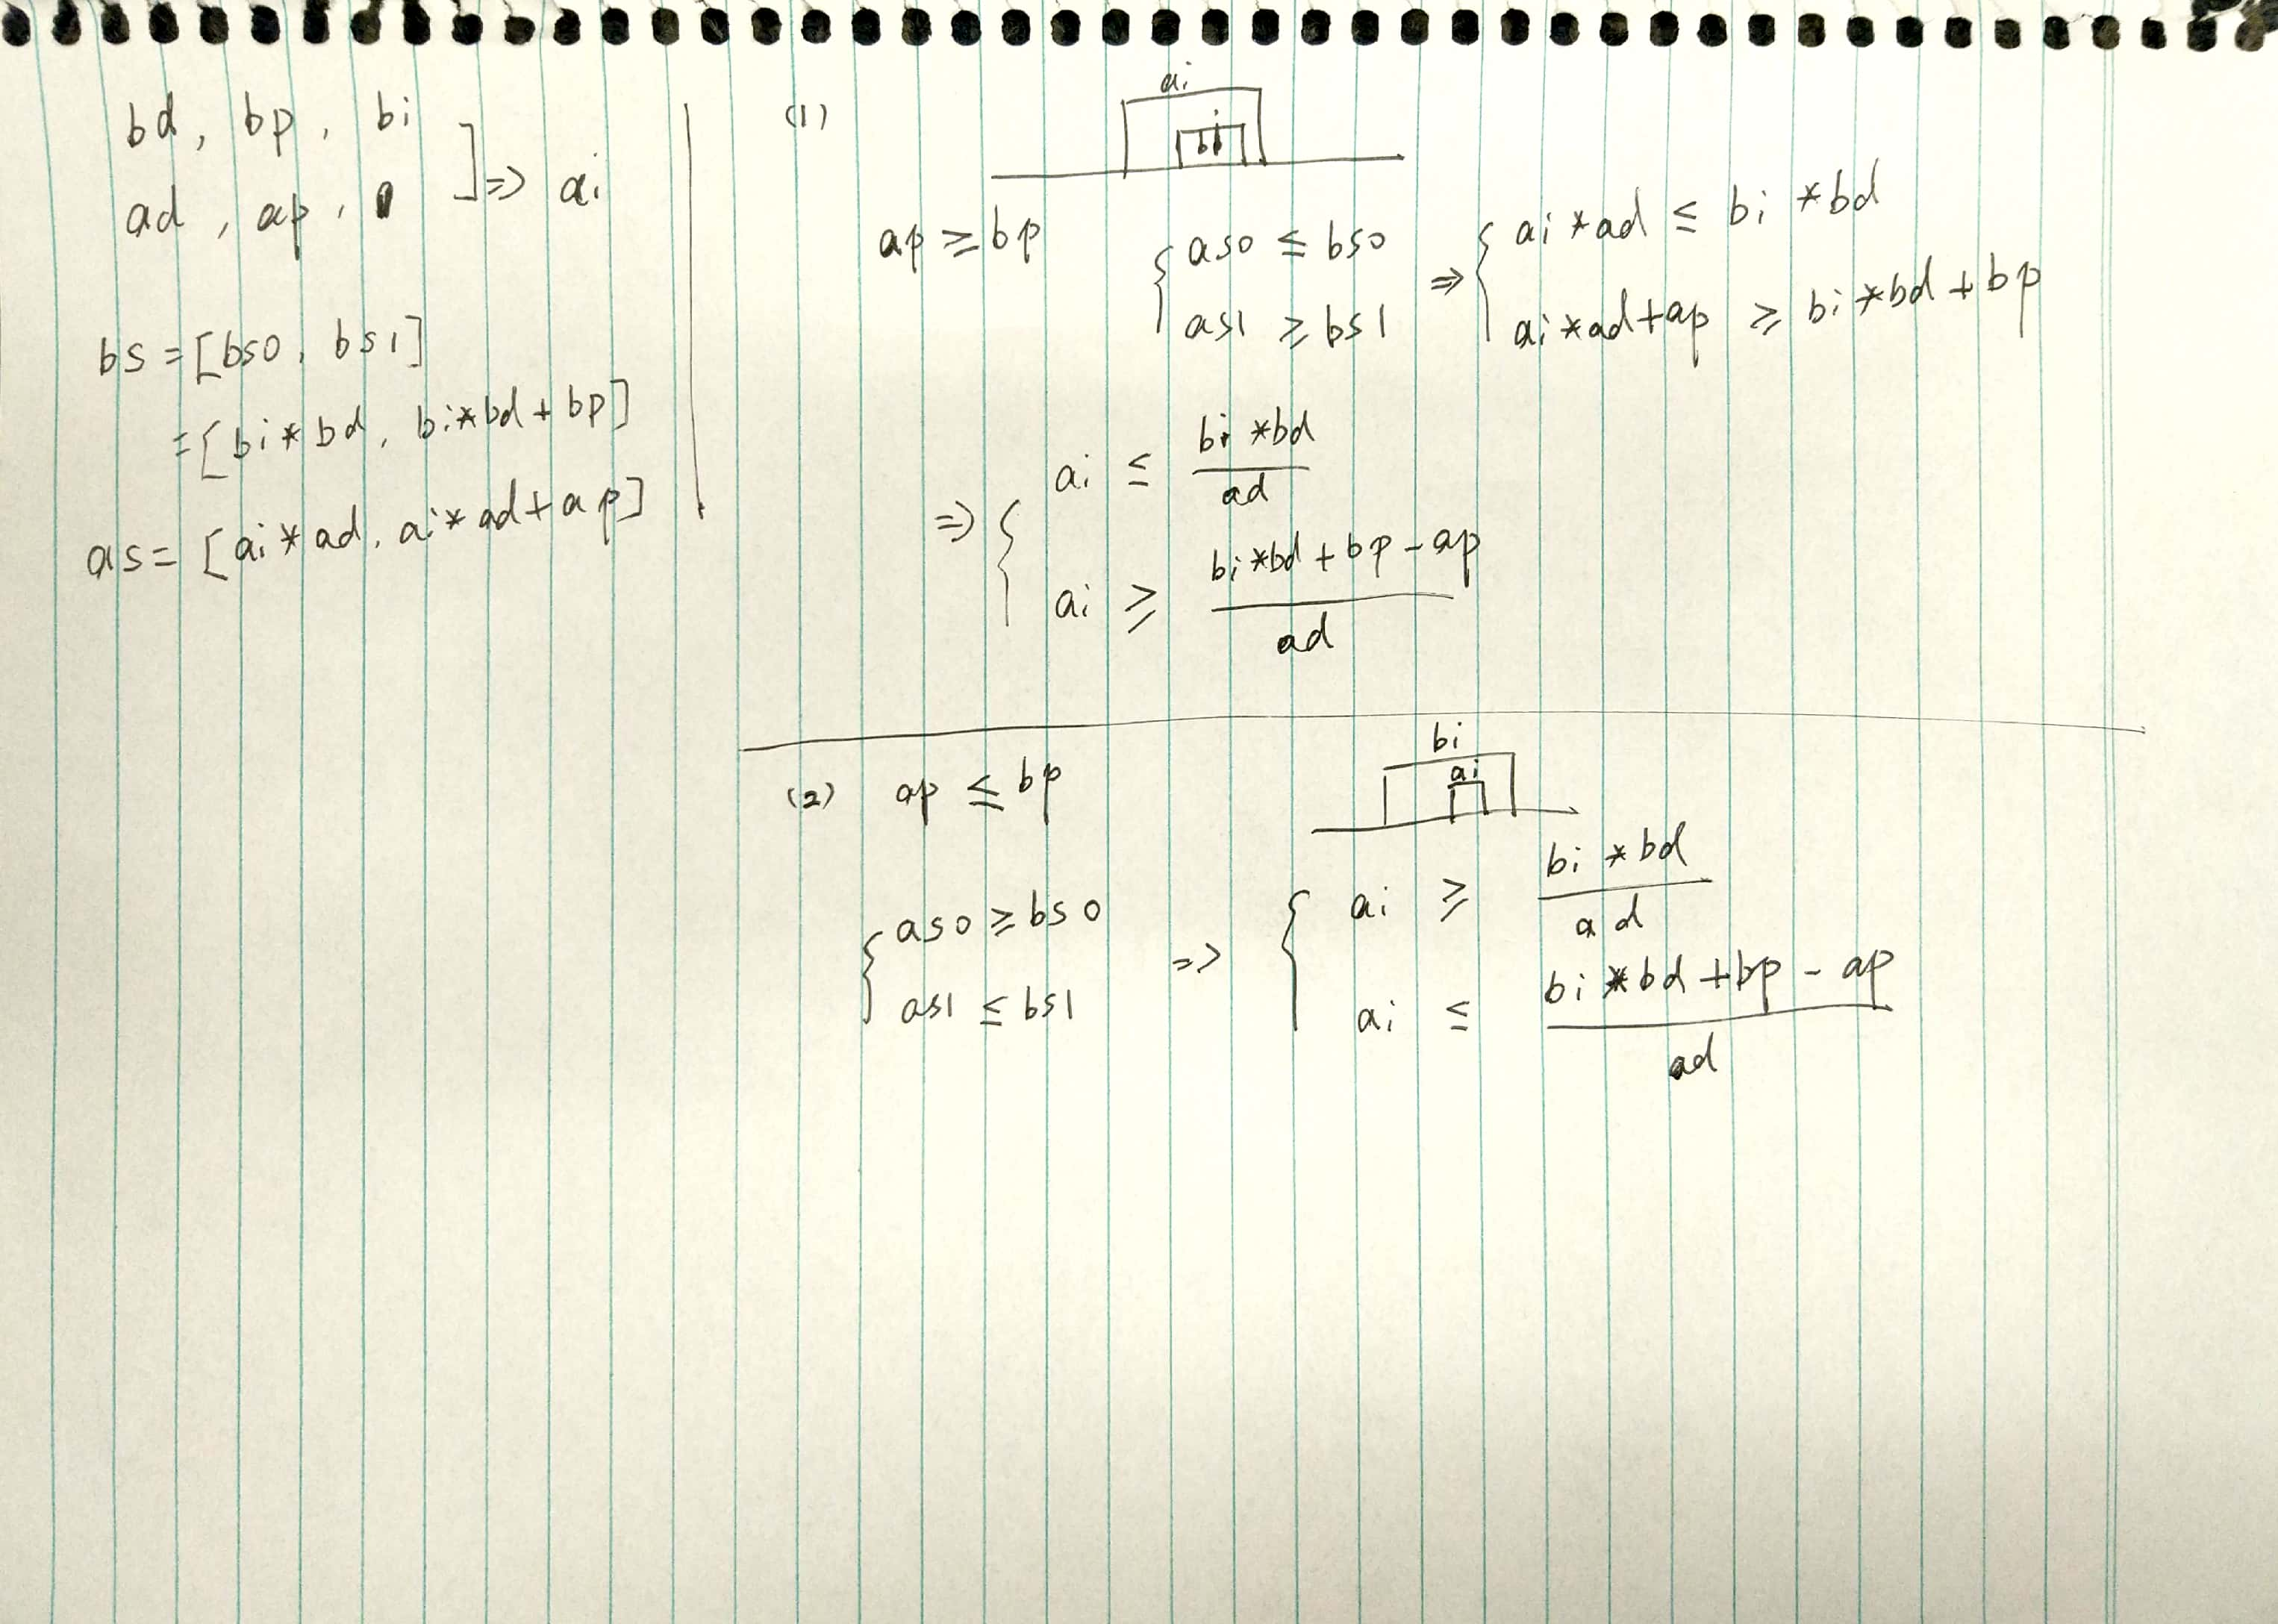
\includegraphics[width=\textheight]{theory/bxmap.png}

\subsubsection{group sampling configuration}
$$ steps = [0.1,0.3,0.9,2.7] + [-6.3]$$
$$ strides = [0.1,0.2,0.6,1.8] + [-3.6] $$
$$ voxel\ size=[, 3, 4, 4, 3] $$
principles:\par
(1)Alignment between differert scales:
$$ steps[i] = steps[i-1]+strides[i-1]*(k-1)\  (k=voxel\ size) $$
(2)Alignment between voxels on one scale:
$$ strides[i] \% steps[i-1] == 0 $$
Examples:\par
$$ 0.3=0.1+0.1*2 \Rightarrow voxel\ size=3 $$
$$ 0.2=0.1*2 $$
$$ 0.9=0.3+0.2*3 \Rightarrow voxel\ size=4 $$ 
$$ 0.6=0.3*2 $$
$$$$
$$ 6.3=2.7+1.8*2 $$
$$ 3.6=1.8*2 $$

\subsubsection{Sparse voxel 3DCNN }
\tikzstyle{startstop} = [rectangle, rounded corners, minimum width=3cm, minimum height=1cm,text centered, draw=black, fill=red!10]
\tikzstyle{io} = [trapezium, trapezium left angle=70, trapezium right angle=110, minimum width=3cm, minimum height=1cm, text centered, draw=black, fill=blue!10]
\tikzstyle{process} = [rectangle, minimum width=3cm, minimum height=1cm, text centered, draw=black, fill=orange!10]
\tikzstyle{decision} = [diamond, minimum width=3cm, minimum height=1cm, text centered, draw=black, fill=green!10]
\tikzstyle{arrow} = [thick,->,>=stealth]

\subsubsection{Data Augmentation} 
\begin{itemize}
\item (1.1) Rotate corrdinate reference: Rotate both point and voxel box \par
Performed by rotating points after sampling and grouping. \par
This should only be applied to point position (cascade 0). What if also to features (upper cascades).

\item (1.2) Rotae point only, or rotate voxel box only. \par
a) It can be performed by rotating points before sampling and grouping.\par
b) If rotate angle is integral times of pi/2, it can be performed by rotating point indices inside the voxel.\par
Rotate voxel can be applied to all cascades.
\item (2.1) Rotate the global block by the same angle
\item (2.2) Rotate each voxel by seperate angle in each scale.\par
Since the features are calculated independently in each voxel, it should be fine to apply different rotatio angle for each voxel. It doesn't matter that the rotation center is voxel center or global block center. It alos doesn't matter that it rotates refference or only rotates voxel.

\end{itemize}

\begin{tikzpicture}[node distance=2cm]
	\node (start) [startstop] {Sparse voxel 3D CNN};
	\node (in) [io, below of=start] {$(b,n_1,c_1)$};
	\node (group) [process, below of=in] {$(b,[g_1]_{n_2},c_1)$};
	\draw [arrow] (in) -- node [anchor=west] {grouping: $g_1$ is inconsistant} (group);
	\node (extend) [process, below of=group] {$(b,n_2,g_{1m},c_1)$};
	\draw [arrow] (group) -- node [anchor=west] {extend: $g_{1m}$ is maximum $g_1$. Tile 0!} (extend);
	\node (transform) [process, below of=extend, align=center] {$(b,n_2,g_{1i},c_1)$ \\ $(b,n_2,d_1,h_1,w_1,c_1)$};
	\draw [arrow] (extend) -- node [anchor=west] {Transform: $g_{1i}$ is the intact number of the voxel} (transform);
	\node (3dconv) [process, below of=transform, align=center] {$(b,n_2,d_{2a},h_{2a},w_{2a},c_{2a})$\\ $(b,n_2,d_{2b},h_{2b},w_{2b},c_{2b})$ \\$(b,n_2,1,1,1,c_2)$};
	\draw [arrow] (transform) -- node [anchor=west] {3D CONV MLP} (3dconv);
	\node (out) [io, below of=3dconv] {$(b,n_2,c_2)$};
	\draw [arrow] (3dconv) -- node [anchor=west] {$n_2$ is the numbel of aim block. Get the feature of each aim block.} (out);
\end{tikzpicture}
\par \par
Two main obstacles for performing 3D convolution on point cloud are: (1) there are too many vacant points, (2) the position of points are not aligned.
The key idea of sparse voxel is to perform 3DCONV on cascades from the second. Because the positions are actually almost aligned. At the same time, the vacant rate within a small block is acceptably large. Above all, it may be possible to do apply 3D-CONV within a small block. 
\par
Centres of blocks in cascades other than first one are actually aligned to the grid. So it is possible to perform 3d convolution directly. However, the average position of points inside these blocks are not aligned. Thus it is also maybe beneficial to utilise a transform net to align them.\par
On the other hand, there are many vacant points in the block. I am wondering if it is beneficial to set the features of vacant points by a T-net from around existing points.
\par

Purpose of T-Net: fix number + align + till \par
There are some interesting problems for Transform net:
\begin{itemize}
	\item Only depend on position or feature.
	\item Should be resolution invariant.
	\item If it should be constant for all channels.
	\item If it should be constant for all local aim blocks.
\end{itemize}
\par
Reasons that we do not need the T-Net:
\begin{itemize}
	\item 3d-conv can till features of the vacant points.
	\item If the base-points are not strictly aligned, add the position to feature map. Or get a special feature of positions within the block and then add ot the main feature map.
\end{itemize}
\par
\begin{tikzpicture}[node distance=2cm]
	\node (start) [startstop] {Transform net: };
	\node (in) [io, below of=start] {$(b,n,g_m,3)$};
	\node (p1) [process, below of=in] {$(b,n,g_m,c_1)$};
	\node (p2) [process, below of=p1] {$(b,n,g_m,c_2)$};
	\node (out) [io, below of=p2] {$(b,n,g_m,g_i)$};
\end{tikzpicture}


\subsection{batch size}
\subsubsection{bs=27 vs bs=81}
batch size: 9,27,81 \par
data: xyz-color\_1norm\par
model: 1AG\par
sampling \& grouping: stride\_0d1\_step\_0d1\_bmap\_nh5\_2048\_0d5\_1\_fmn1-160\_32-32\_12-0d2\_0d6-0d2\_0d6\par
\begin{figure}[h!]
	\caption{bs=9}
	\centering
	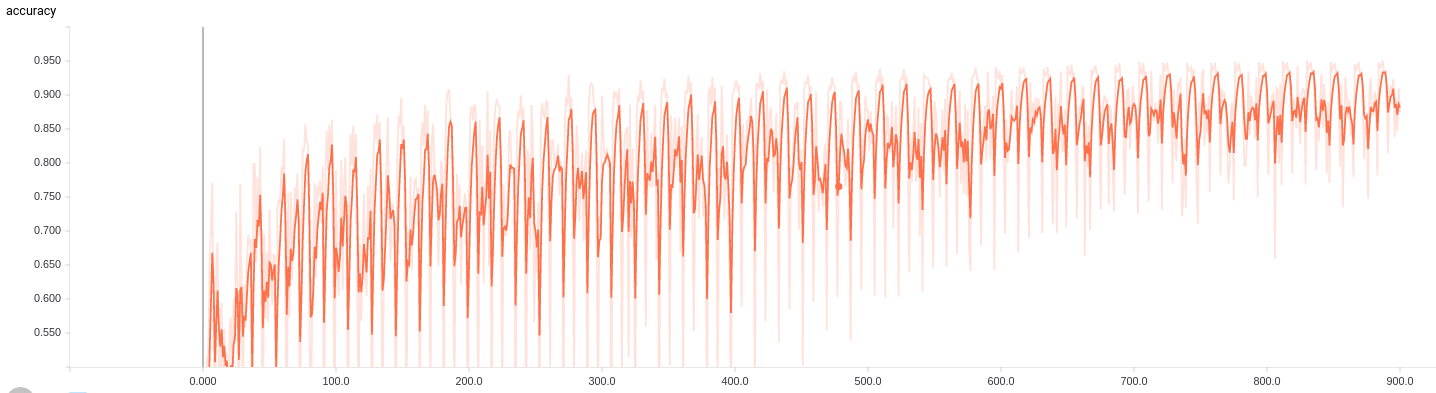
\includegraphics[width=\textwidth]{acc_log-model_1AG-gsbb_2C1-bs9-xyz-color_1norm-2048-mat}
	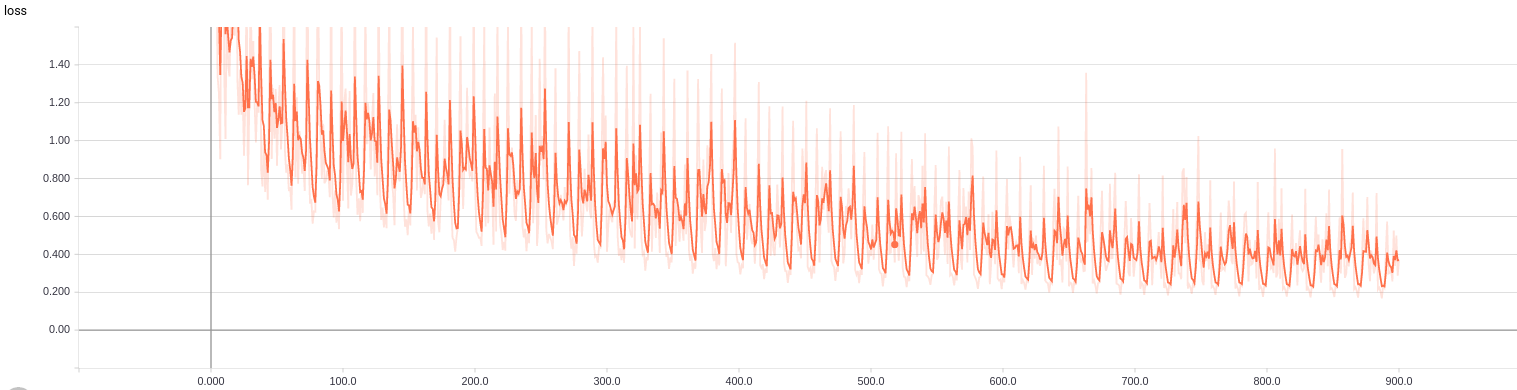
\includegraphics[width=\textwidth]{loss_log-model_1AG-gsbb_2C1-bs9-xyz-color_1norm-2048-mat}
\end{figure}
\begin{figure}[h!]
	\caption{bs=27}
	\centering
	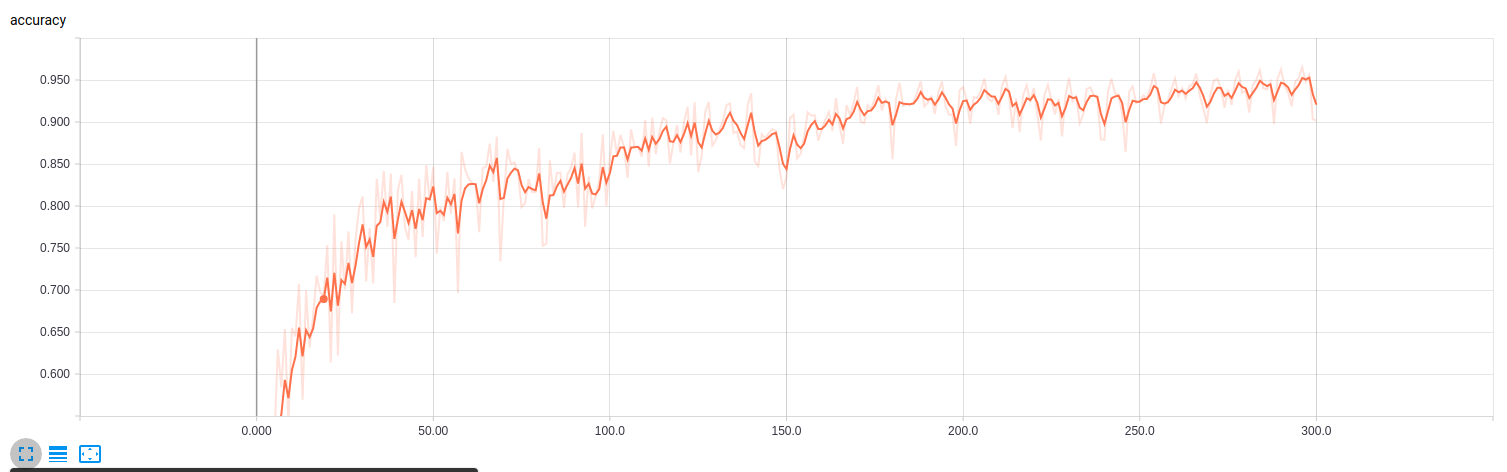
\includegraphics[width=\textwidth]{acc_log-model_1AG-gsbb_2C1-bs27-xyz-color_1norm-2048-mat}
	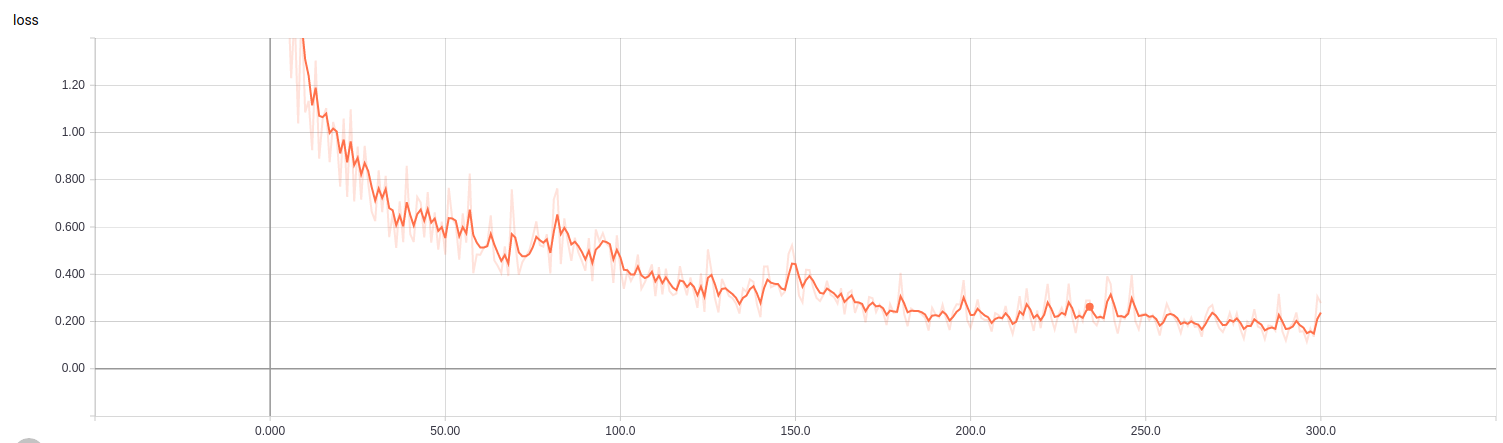
\includegraphics[width=\textwidth]{loss_log-model_1AG-gsbb_2C1-bs27-xyz-color_1norm-2048-mat}
\end{figure}
\begin{figure}[h!]
	\centering
	\caption{bs=81}
	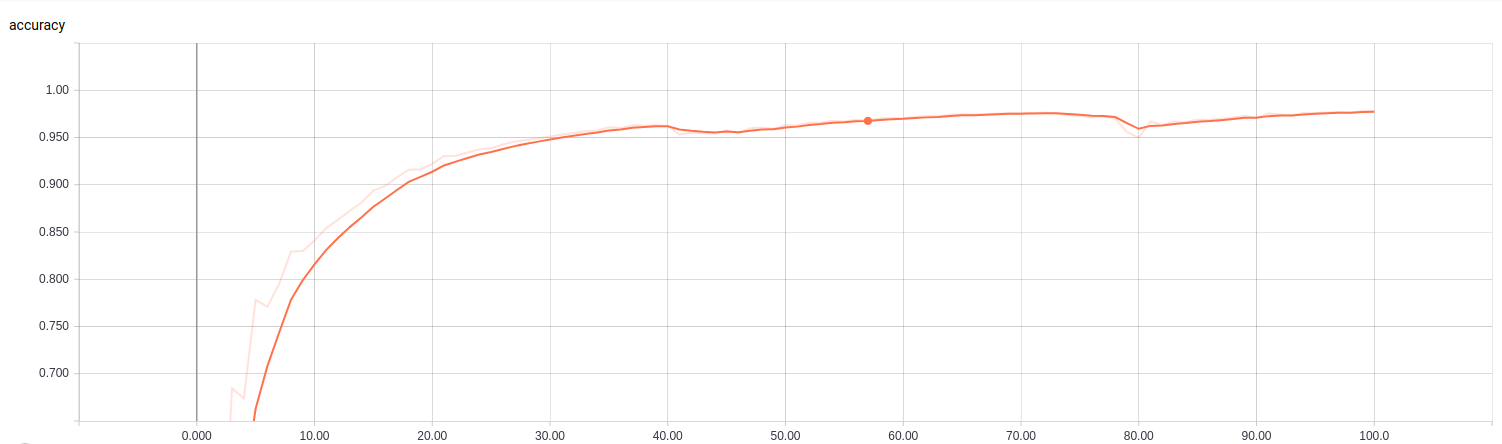
\includegraphics[width=\textwidth]{acc_log-model_1AG-gsbb_2C1-bs81-xyz-color_1norm-2048-mat}
	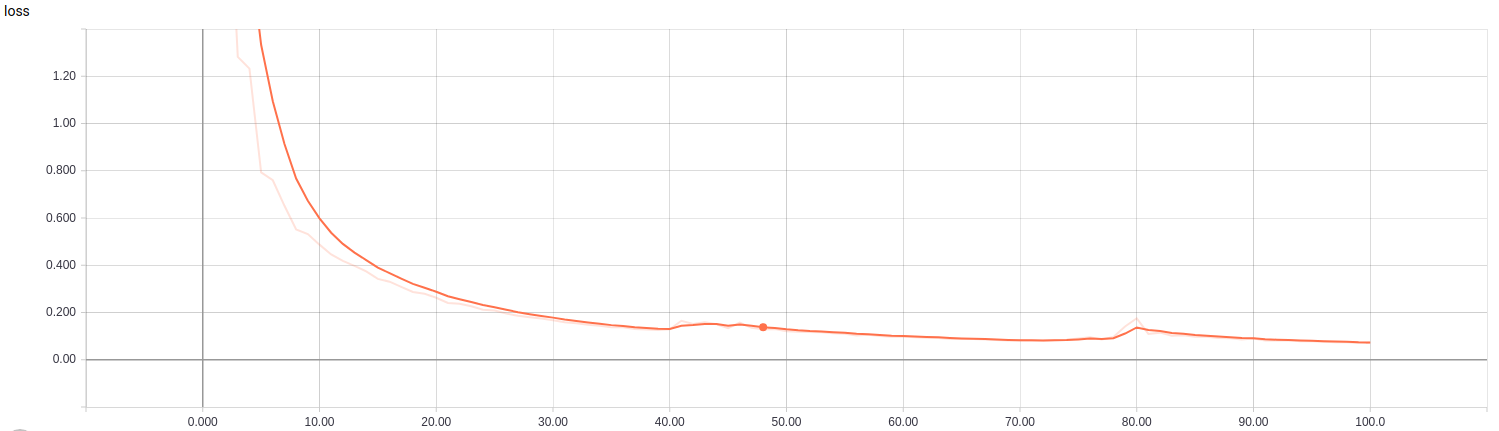
\includegraphics[width=\textwidth]{loss_log-model_1AG-gsbb_2C1-bs81-xyz-color_1norm-2048-mat}
\end{figure}

\subsection{feed elements}
epoch num = 100 \par
stride\_0d1\_step\_0d1\_bmap\_nh5\_2048\_0d5\_1\_fmn1-160\_32-32\_12-0d2\_0d6-0d2\_0d6 \par
\begin{center}
	\begin{tabular}{|c |c | c || c c |} 
		\hline
		model & batch size & data elements & acc & loss \\
		\hline
		1AG & 9 & xyz color & 0.890 & 0.356\\ [0.5ex] 
		\hline
		1AG & 27 & xyz color & 0.920 & 0.240\\ [0.5ex] 
		\hline
		
		3AG & 27 & xyz color& 0.912 & 0.273 \\  [0.5ex]
		\hline
		2A & 27 & xyz color& 0.908 & 0.294 \\  [0.5ex]
		\hline
		2AG & 27 & xyz color& 0.902 & 0.293 \\  [0.5ex]
		\hline
		1A & 27 & xyz color& 0.883 & 0.351 \\  [0.5ex]
		\hline
		1AG & 81 & xyz color & 0.978 & 0.072\\ [0.5ex] 
		\hline\hline
		
		1AG & 9 & xyz  & 0.861 & 0.427\\ [0.5ex] 
		\hline
		1AG & 27 & xyz & 0.907 & 0.257\\ [0.5ex] 
		\hline
		1AG & 81 & xyz & 0.975 & 0.078 \\  [0.5ex]
		\hline\hline
		1A & 27 & xyzmid color& 0.889 & 0.357 \\  [0.5ex]
		\hline
		3AG & 27 & xyzmid color& 0.933 & 0.193 \\  [0.5ex]
		\hline
		
		2A & 27 & xyzmid color& 0.939 & 0.177 \\  [0.5ex]
		\hline
		
		2AG & 27 & xyzmid color& 0.929 & 0.208 \\  [0.5ex]
		\hline\hline
		3AG & 27 & xyz xyzmid color& 0.924 & 0.230 \\  [0.5ex]
		\hline
		
		2A & 27 & xyz xyzmid color& 0.898 & 0.317 \\  [0.5ex]
		\hline
		2AG & 27 & xyz xyzmid color& 0.908 & 0.280 \\  [0.5ex]
		\hline
		1A & 27 & xyz xyzmid color& 0.910 & 0.281 \\  [0.5ex]
		\hline
		1AG & 27 & xyz xyzmid color& 0.944 & 0.163 \\  [0.5ex]
		\hline
		1AG & 81 & xyz xyzmid color& 0.976 & 0.078 \\  [0.5ex]
		\hline
		2A & 81 & xyz xyzmid color& 0.942 & 0.173 \\  [0.5ex]
		\hline
		3AG & 81 & xyz xyzmid color& 0.949 & 0.147 \\  [0.5ex]
		\hline
	\end{tabular}
\end{center}

1. large batch size is better \par
2. $1AG (0.92) > 3AG(0.912) > 2A(0.908) > 2AG(0.902) > 1A(883)$ \par
   1AG is much better than 1A \par 
   \textbf{1AG is a bit better than 3AG ???} \par

3. xyz-color is only a bit better than xyz \par
4. xyzmid-color is much better than xyz-color \par
5. \textbf{xyzmid-color is normally much better than xyz-xyzmid-color ???} \par



\subsection{model}
batch size: 50 \par
data: xyz\_midnorm\_block-color\_1norm \par
epoch\_num = 600 \par
sampling \& grouping: stride\_0d1\_step\_0d1\_bmap\_nh5\_12800\_1d6\_2\_fmn3-600\_64\_24-60\_16\_12-0d2\_0d6\_1d2-0d2\_0d6\_1d2 \par
\begin{center}
	\begin{tabular}{|c | c c |} 
		\hline
		model  & acc & loss \\
		\hline
		3A & 0.909 & 0.248 \\ [0.5ex] 
		\hline
		3AG & 0.913 & 0.231 \\ [0.5ex] 
		\hline
		4AG & 0.912 & 0.232 \\ [0.5ex] 
		\hline	
	\end{tabular}
\end{center}

batch size: 32 \par
data: xyz\_midnorm\_block-color\_1norm \par
sampling \& grouping: stride\_0d1\_step\_0d1\_bmap\_nh5\_12800\_1d6\_2\_fmn6-2048\_256\_64-32\_32\_16-0d2\_0d6\_1d2-0d1\_0d3\_0d6 \par
matterport3d  \par
feed\_data\_elements:['xyz\_midnorm\_block', 'color\_1norm']  \par
feed\_label\_elements:['label\_category', 'label\_instance']  \par
train data shape: [  362 12800     6]  \par  
test data shape: [  384 12800     6] \par
max epoch = 500
\begin{center}
	\begin{tabular}{|c | c c |} 
		\hline
		model  & acc & loss \\
		\hline
		1AG & 0.944/0.431 & 0.161/4.633 \\ [0.5ex] 
		\hline
		
		4AG & 0.835/0.401 & 0.520/3.644 \\ [0.5ex] 
		\hline	
	\end{tabular}
\end{center}

\subsection{integration: matterport3d}
\begin{center}
	\centering \def\arraystretch{1.5} \small
	\begin{longtable}{|p{1cm} |p{1.5cm} | p{2cm} | p{3.5cm} || p{4cm}|} 
		\hline
		\multicolumn{5}{|c|}{stride\_0d1\_step\_0d1\_bmap\_nh5\_12800\_1d6\_2\_fmn3-512\_64\_24-48\_16\_12-0d2\_0d6\_1d2-0d2\_0d6\_1d2 }\\
		\multicolumn{5}{|c|}{17D\_1LX\_1pX\_29h\_2az}\\
		\hline
		model & batch size\par batch num \par shuffle& lr\par ds & data elements & epoch-acc mean-std \par train/eval \\
		\hline
		1aG & 30/60 & 0.005 & 'xyz\_midnorm\_block', 'color\_1norm', 'nxnynz'& 250-0.981  \\  [0.5ex]
		\hline
		1DSaG & 30/60 & 0.001-40 & 'xyz\_midnorm\_block', 'color\_1norm', 'nxnynz'& 300-0.914-0.775  \\  \hline
		1DSaG & 30/60 & 0.001-40 & 'xyz\_midnorm\_block', 'color\_1norm', 'nxnynz'& 300-0.914-0.775  \\  [0.5ex] \hline
		1DSaG \par kp0.5& 30/60 & 0.001-80\par 300-3e-4 & 'xyz\_midnorm\_block', 'color\_1norm', 'nxnynz'& 300-0.942-0.842  \\  [0.5ex] \hline
		1DSaG \par kp0.2& 30/60 & 0.001-80\par 300-3e-4 & 'xyz\_midnorm\_block', 'color\_1norm', 'nxnynz'& 300-0.928-0.797  \\  [0.5ex] \hline
		1DSaG \par kp0.5& 30/60 & 0.005-80\par 300-1.7e-3 & 'xyz\_midnorm\_block', 'color\_1norm', 'nxnynz'& 300-0.970-0.916  \\  [0.5ex] \hline
		1DSaG \par kp0.2& 30/60 & 0.005-80\par 300-1.7e-3 & 'xyz\_midnorm\_block', 'color\_1norm', 'nxnynz'& 300-0.966-0.924  \\  [0.5ex] \hline
		1DSaG \par kp0.8& 30/60 & 0.005-80\par 300-1.7e-3 & 'xyz\_midnorm\_block', 'color\_1norm', 'nxnynz'& 300-0.976-0.933 \par 500-0.984-0.954 \\  [0.5ex] \hline
		
		
		\hline\hline
		1aG & 30/1083 & 0.003 & 'xyz\_midnorm\_block', 'color\_1norm', 'nxnynz'& 200-0.947  \\  [0.5ex]
		\hline		
		1aG & 30/1083 & 0.01  & 'xyz\_midnorm\_block', 'color\_1norm'& 200-0.783 \par 500-0.791  \\  [0.5ex]
		\hline		
		1aG & 30/1083 & 0.003/30 \par 300-0.00012 & 'xyz\_midnorm\_block', 'color\_1norm'& 200-0.903 \par 300-0.921  \\  [0.5ex]
		\hline\hline
		
		1bG & 25/1083 & 0.001-30 \par 100-3e-4 \par 300-4e-5 & 'xyz\_midnorm\_block'& 100-0.854 \par 200-0.918 \par 300-0.936  \\  [0.5ex]
		\hline
		1bG & 25/1083 & 0.001-30 \par 100-3e-4 \par 300-4e-5 & 'xyz\_midnorm\_block', 'color\_1norm', 'nxnynz'& 100-0.914 \par 200-0.957 \par 300-0.966  \\  [0.5ex]
		\hline	
		1bG & 25/1083 & 0.02 & 'xyz\_midnorm\_block', 'color\_1norm'& 200-0.655 \par 300-0.718  \\  [0.5ex]
		\hline
		1bG & 25/1083 & 0.02 & 'xyz\_midnorm\_block', 'color\_1norm', 'nxnynz'& 200-0.772 \par 300-0.823  \\  [0.5ex]
		\hline
		1bG & 25/1083 & 0.001 & 'xyz'& 200-0.772 \par 90-0.553-0.210  \\  [0.5ex]
		\hline \hline
		
		
		4bG & 25/1083 & 0.001-30 \par 100-3e-4 \par 200-1e-4 \par 300-4e-5& 'xyz\_midnorm\_block', 'color\_1norm', 'nxnynz'& 100-0.752 \par 200-0.816 \par 300-0.832  \\  [0.5ex] \hline2
		
		1DSaG & 30/1083 & 0.002-80 & 'xyz\_midnorm\_block', 'color\_1norm', 'nxnynz'& 200-0.930-0.830/0.450 \par 460-0.952-0.881/0.471 \\  [0.5ex] \hline
		
		\hline \hline
		1aG & 30/19755 & 0.001-30 \par 50-7e-4 \par 100-3e-4& 'xyz\_midnorm\_block', 'color\_1norm','nxnynz'& 50-0.752/0.580 \par 100-0.843/0.574 (\colorbox{Yellow}{NoShuf}) \par 102-0.806/0.570 (\colorbox{Yellow}{Shufle})   \\  [0.5ex]
		\hline
		1bG & 25/19755 & 0.001-30& 'xyz\_midnorm\_block', 'color\_1norm','nxnynz'& 38-0.719/0.587 \par 80-0.823/0.583 (\colorbox{Yellow}{NoShuf}) \par 81-0.782/0.587 (\colorbox{Yellow}{Shufle}) \\  [0.5ex]
		\hline
		1aG & 30/19755 & 0.02 & 'xyz\_midnorm\_block', 'color\_1norm'& 56-0.562   \\  [0.5ex]
		\hline
		1aG & 30/19755 & 0.02 \par 127-0.00483& 'xyz\_midnorm\_block', 'color\_1norm', 'nxnynz'& 87-0.616 \par 127-0.686 \\  [0.5ex]
		\hline
		\hline
		1bG & 25/18737 & 0.001 \par N& 'xyz\_midnorm\_block', 'color\_1norm', 'nxnynz'& 24-0.682/0.509 \par 70-0.858/0.509\\  [0.5ex]
		\hline
		1bG & 25/18737 & 0.001 \par Y& 'xyz\_midnorm\_block', 'color\_1norm', 'nxnynz'& 24-0.738/0.573 \par 70-0.876/0.563 \par \colorbox{Yellow}{90-0.897}/0.561\\  [0.5ex]
		\hline
		4bG & 25/18737 & 0.001 \par Y& 'xyz\_midnorm\_block', 'nxnynz'& 24-0.576/0.545 \\  [0.5ex]
		
		\hline
		4bG & 25/18737 & 0.001 \par Y& 'xyz\_midnorm\_block', 'color\_1norm', 'nxnynz'& 24-0.594/0.569 \\  [0.5ex]
		\hline
		1DSaG & 30/18737 & 0.002-80 \par Y& 'xyz\_midnorm\_block', 'color\_1norm', 'nxnynz'& 20-0.688-0.394/0.428-0.224 \par 36-0.742/0.395 \\  [0.5ex]
		\hline
		1DSaG & 30/18737 & 0.007-80 \par Y& 'xyz\_midnorm\_block', 'color\_1norm', 'nxnynz'& 20-0.725-0.453/0.435-0.206 \par 38-0.783/0.396 \\  [0.5ex]
		\hline
		\multicolumn{5}{|l|}{ \shortstack[l]{Conclusion:\\ 
				1: nxnynz helps a lot \\
				2: 1bG is much deeper than 1aG, why worse than 1aG \\
				3: learning rate is important, cannot be too large
		} }  \\
		\hline
	\end{longtable}
\end{center}

\subsection{multi scales \& mat 1083}
\begin{tabular}{|p{1.5cm}|p{1.5cm}|p{1cm}|p{2cm}|p{1cm}|p{6cm}| }
	\hline
	\multicolumn{6}{|p{12cm}|}{nh5: stride\_0d1\_step\_0d1\_pl\_nh5-1d6\_2/17D\_1LX\_1pX\_29h\_2az\par bxmh5: stride\_0d1\_step\_0d1\_bxmh5-12800\_1d6\_2\_fmn4-480\_80\_24-80\_20\_10-0d2\_0d6\_1d2-0d2\_0d6\_1d2-3A1} \\		
	\hline
	model & bs/bn& lr-decay & elements & loss weight\par in drop & epoch-pacc-cacc train/eval \\
	\hline
	4bG\_111 & 20/1083 &2-40 & xyz\_midnorm\_block-color\_1norm-nxnynz & E &110-0.898-0.763\par 160-0.931-0.827 \par 300-0.967-0.915 \\
	\hline
	4bG\_444 & 15/1083 &3-40 & xyz\_midnorm\_block-color\_1norm-nxnynz & E &60-0.729-0.614\par 100-0.857-0.721\par 160-0.920-0.834\par 260-0.952-0.890\par 300-0.958-0.913 \\
	\hline
	4bG\_444 & 15/1083 &2-40 & xyz\_midnorm\_block-color\_1norm-nxnynz & E &60-0.778-0.608\par 100-0.878-0.758\par 160-0.930-0.838\par 260-0.957-0.901\par 300-0.964-0.912 \\
	\hline
	4bG\_144 & 18/1083 &2-40 & xyz\_midnorm\_block-color\_1norm-nxnynz & E &60-0.786-0.637\par 100-0.876-0.767\par 160-0.926-0.820\par 260-0.959-0.885\par 300-0.962-0.906 \\
	\hline
	4bG\_114 & 20/1083 &2-40 & xyz\_midnorm\_block-color\_1norm-nxnynz & E &60-0.772-0.611\par 100-0.874-0.764\par 160-0.926-0.851\par 260-0.958-0.893 /par 300-0.963-0.904 \\
	\hline
	3aG\_444 & 45/1083 &2-40 & xyz\_midnorm\_block-color\_1norm-nxnynz & E &60-0.893-0.737\par 100-0.908-0.786 /par 160-0.934-0.833\par 260-0.950-0.868 /par 300-0.952-0.882 \\
	\hline
	2aG\_144 & 30/1083 &2-40 & xyz\_midnorm\_block-color\_1norm-nxnynz & E &60-0.890-0.754\par 100-0.922-0.820 /par 160-0.942-0.858:\par 260-0.957-0.897 /par 300-0.960-0.911 \\
	\hline	
\end{tabular}

\subsection{multi scales \& mat 21826}
\begin{tabular}{|p{1.5cm}|p{1.5cm}|p{1cm}|p{2cm}|p{1.5cm}|p{6cm}| }
	\hline
	\multicolumn{6}{|p{12cm}|}{nh5: stride\_0d1\_step\_0d1\_pl\_nh5-1d6\_2/ \par bxmh5:  stride\_0d1\_step\_0d1\_bxmh5-12800\_1d6\_2\_fmn4-480\_80\_24-80\_20\_10-0d2\_0d6\_1d2-0d2\_0d6\_1d2-3A1 \par eval: 17D\_1LX\_1pX\_29h\_2az } \\
	\hline
	model & bs/bn& lr-decay & elements & loss weight\par in drop & epoch-pacc-cacc train/eval \\
	\hline
	4bG\_114 & 20/1080 &1-30 & xyz midnorm\par color\par nxnynz & E\par N &40-0.784-0.545/0.579-0.451 \par 80-0.883-0.699/0.584-0.439 \par 140-0.925-0.795/0.575-0.429 \\
	\hline
	4bG\_111 & 20/1080 &2-30 & xyz midnorm\par color\par nxnynz & E\par N &40-0.737-0.489/0.587-0.412\par 80-0.836-0.614/0.582-0.411 \par 95-0.867/0.588 \\
	\hline 
	4bG\_144 & 20/1200 &2-30 & xyz midnorm\par color\par nxnynz & E\par N &40-0.761-0.543/0.601-0.416\par 80-0.864-0.693/0.602-0.426 \par 95-0.888/0.597 \\
	\hline
	 
	\multicolumn{6}{|p{12cm}|}{ Conclusion:\par	(1) Nein 114 is better than 111  } \\
	\hline
\end{tabular}	

\subsection{multi scales \& scannet 12887}
\begin{tabular}{|p{1.5cm}|p{1cm}|p{1cm}|p{2cm}|p{1cm}||p{5cm}| }
	\hline
	\multicolumn{6}{|p{12cm}|}{nh5: stride\_0d1\_step\_0d1\_pl\_nh5-1d6\_2/ \par bxmh5:  stride\_0d1\_step\_0d1\_bxmh5-12800\_1d6\_2\_fmn4-480\_80\_24-80\_20\_10-0d2\_0d6\_1d2-0d2\_0d6\_1d2-3A1
	\par eval: test } \\		
	\hline
	model & bs/bn& lr-decay & elements & loss weight\par in drop & epoch-pacc-cacc train/eval \\
	\hline
	2aG\_144 & 30/420 &2-30 & xyz midnorm & E\par N &40-0.833-0.546/0.686-0.89 \par 100-0.926-0.727/0.683-0.326\\
	\hline
	3aG\_144 & 48/260 &2-30 & xyz midnorm & E\par N &40-0.841-0.530/0.668-0.346 \par 100-0.924-0.709/0.673-0.327\par 200-0.949-0.782/0.673-0.332 \par \textbf{300-0.955-0.802/0.671-0.330} \\
	\hline 
	4bG\_111 & 22-580 & 2-30 & xyz midnorm & E \par N &60-0.738-0.434/0.706-0.344 \par 100-0.796-0.506/0.699-0.315\par 180-0.863-0.589/0.695-0.308 \\
	\hline
	4bG\_111 & 22-580 & 7-30 & xyz midnorm & E \par N &60-0.705-0.378/0.684-0.362 \\
	\hline
	4bG\_144 & 18-700 & 2-30 & xyz midnorm & E \par N &40-0.714-0.470/0.6910.433\par 100-0.794-0.481/0.682-0.393\par 160-0.849-0.582/0.676-0.362 \\
	\hline
	4aG\_1a4 & 55-220 & 2-30 & xyz midnorm & CN \par N &40-0.775-0.482/0.654-0.304\par 100-0.877-0.637/0.661-0.298\par 160-0.901-0.690/0.660-0.311 \par 220-0.908-0.707/0.655-0.334\\
	\hline
	4aG\_1a4 & 55-220 & 2-30 & xyz midnorm & E \par N &40-0.819-0.527/0.684-0.333\par 100-0.923-0.706/0.681-0.304\\
	
	\hline\hline
	\multicolumn{6}{|p{12cm}|}{ Conclusion:\par	(1) 3aG is much better than 4bG. Potential reasons:(a) 4bG is too wide and deep, so that needs more time to train. (b) The batch size of 4bG is too small \par (2) nein 144 seems is not better than 111 \par (3)Learning rate 0.002 is better than 0.007 \par (4)Loss weight CN does not help} \\
	\hline
\end{tabular}	

\subsection{integration: scannet}
\begin{center}
	\centering \def\arraystretch{1.5} \small
	\begin{tabular}{|p{1cm} |p{1cm} |p{1.5cm} | p{2cm} | p{2cm} || p{5cm}|} 
		\hline
		\multicolumn{6}{|c|}{stride\_0d1\_step\_0d1\_bmap\_nh5\_12800\_1d6\_2\_fmn3-256\_48\_16-56\_8\_8-0d2\_0d6\_1d2-0d2\_0d6\_1d2 }\\
		\multicolumn{6}{|c|}{ scannet train }\\
		\hline
		model & loss: E,N,C \par input drop (No) & batch size\par batch num \par shuffle& lr\par ds & data elements & epoch-point ac-class ac \par train/eval \\
		\hline
		1bG & E & 25/12887\par test \par Y & 0.001\par 40 & xyzmid & 23-0.732-0.326/0.664-0.260 \par 25-0.746-0.340/0.669-0.273\\ \hline
		1bG & N & 25/12887\par Y & 0.001\par 40 & xyzmid & 25-0.733-0.390/0.666-0.252\\ \hline
		1bG & C & 25/12887\par Y & 0.001\par 40 & xyzmid & 25-0.703-0.356/0.655-0.252\\ \hline
		1bG & CN & 25/12887\par Y & 0.001\par 40 & xyzmid & 25-0.681-0.366/0.611-0.237\\ \hline
		1DSaG & E \par idp9& 30/12887\par Y & 0.003\par 80 & xyzmid & 40-0.738-0.376/0.513-0.228 \par 90-0.832/0.496\\ \hline
		
		
		\hline\hline
		1bG & E & 25/13091\par train\_300\par Y & 0.002\par 80 & xyzmid & 60-0.765-0.389/0.700-0.252\\ \hline
		1bG & E & 25/13091\par Y & 0.003\par 80 & xyzmid & 10-0.646/0.689 \par 60-0.753-0.349/0.691-0.234 \par  100-0.833-0.480/0.672-0.261\\ \hline
		1bG & CN & 25/13091\par Y & 0.002\par 80 & xyzmid & 60-0.738-0.409/0.670-0.237\\ \hline
		1bG & E \par idp9 & 25/13091\par Y & 0.003\par 80 & xyzmid & 10-0.641/0.585 \par 16-0.646/0.633\\ \hline
		1DSaG & E & 30/13091\par Y & 0.003\par 80 & xyzmid & 40-0.794-0.456/0.420-0.154 \par 100-0.872-0.602/0.417-0.153\\ \hline
		
		\multicolumn{6}{|p{12.5cm}|}{ Conclusion:\par		 }  \\
		
		\hline\hline
		4bG & CN & 25/2998-3521\par Y & 0.001\par 40 & xyzmid & 142-0.726-0.445/0.625-0.242\\
		\hline
		4bG & E & 25/2998-3521\par Y & 0.001\par 40 & xyzmid & 145-0.792-0.506/0.656-0.257\\
		\hline
	\end{tabular}
\end{center}


\subsection{Semantic segmentation expamples}
\subsubsection{good: 1083, train, 0.946}
log: log-model\_1bG-gsbb\_3B1-bs25-lr1-ds\_30-xyz\_midnorm\_block-color\_1norm-nxnynz-12800-mat\_1083 \par
model: 1bG \par
sampling \& grouping: \par stride\_0d1\_step\_0d1\_bmap\_nh5\_12800\_1d6\_2\_fmn3-512\_64\_24-48\_16\_12-0d2\_0d6\_1d2-0d2\_0d6\_1d2 \par
batch size: 25 \par
learning rate: 0.001000 \par
decay\_epoch\_step: 30 \par
matterport3d  \par
feed\_data\_elements:['xyz\_midnorm\_block', 'color\_1norm', 'nxnynz']  \par
feed\_label\_elements:['label\_category', 'label\_instance']  \par
train data shape: [ 1083 12800     9] \par

\begin{figure}[H]
	\centering
	\begin{subfigure}[h]{0.49\textwidth}
	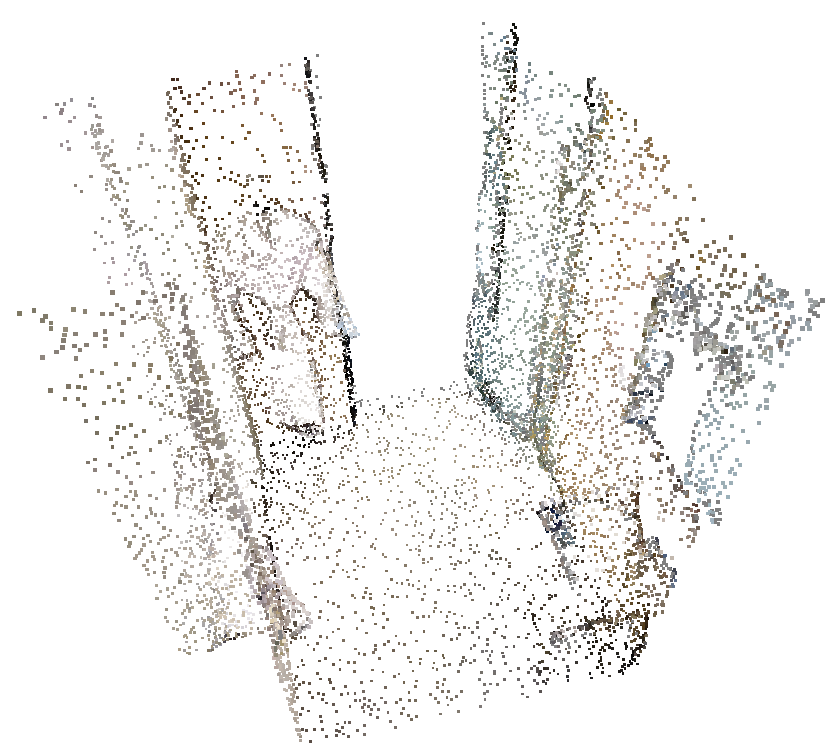
\includegraphics[width=\textwidth]{ply_log-model_1bG-gsbb_3B1-bs25-lr1-ds_30-xyz_midnorm_block-color_1norm-nxnynz-12800-mat_1083/17DRP5sb8fy_1_2_a946/raw00.png}
	\caption{colorized point cloud}
	\end{subfigure}
	\begin{subfigure}[h]{0.49\textwidth}
	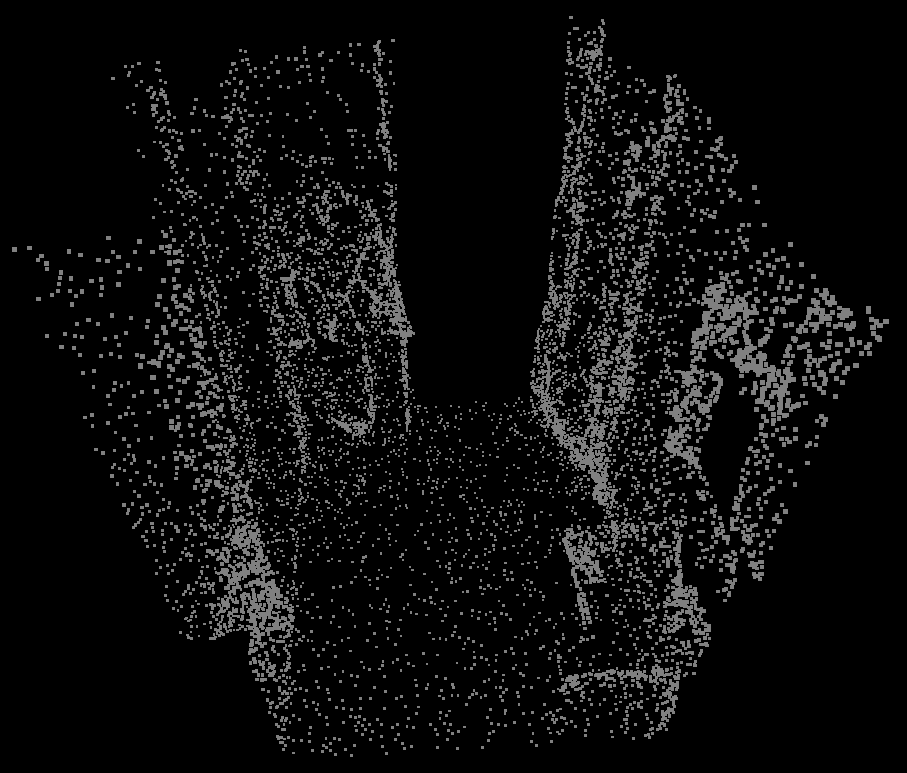
\includegraphics[width=\textwidth]{ply_log-model_1bG-gsbb_3B1-bs25-lr1-ds_30-xyz_midnorm_block-color_1norm-nxnynz-12800-mat_1083/17DRP5sb8fy_1_2_a946/xyz00.png}
	\caption{raw point cloud}
	\end{subfigure}
	\begin{subfigure}[h]{0.5\textwidth}
	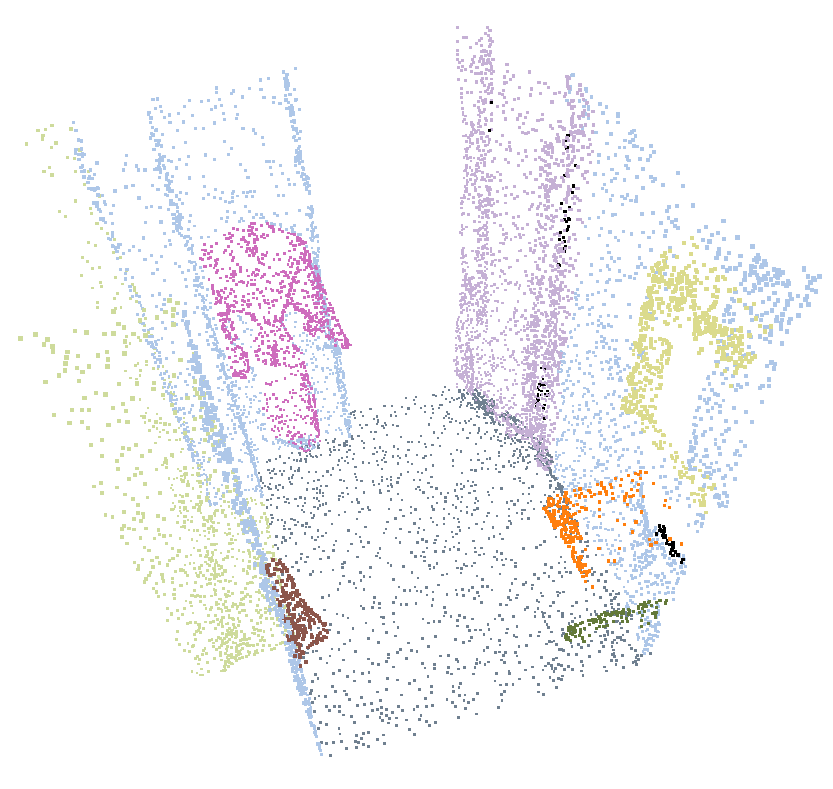
\includegraphics[width=\textwidth]{ply_log-model_1bG-gsbb_3B1-bs25-lr1-ds_30-xyz_midnorm_block-color_1norm-nxnynz-12800-mat_1083/17DRP5sb8fy_1_2_a946/gt00.png}
	\caption{gt}
	\end{subfigure}
	\begin{subfigure}[h]{0.49\textwidth}
	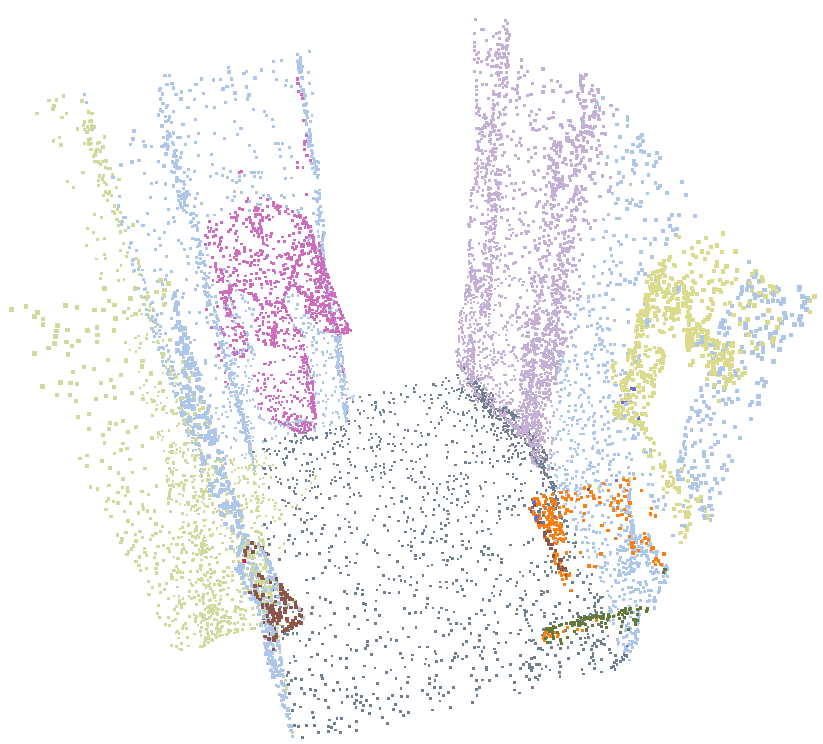
\includegraphics[width=\textwidth]{ply_log-model_1bG-gsbb_3B1-bs25-lr1-ds_30-xyz_midnorm_block-color_1norm-nxnynz-12800-mat_1083/17DRP5sb8fy_1_2_a946/pred00.png}	
	\caption{pred}
	\end{subfigure}
	\begin{subfigure}[h]{0.5\textwidth}
	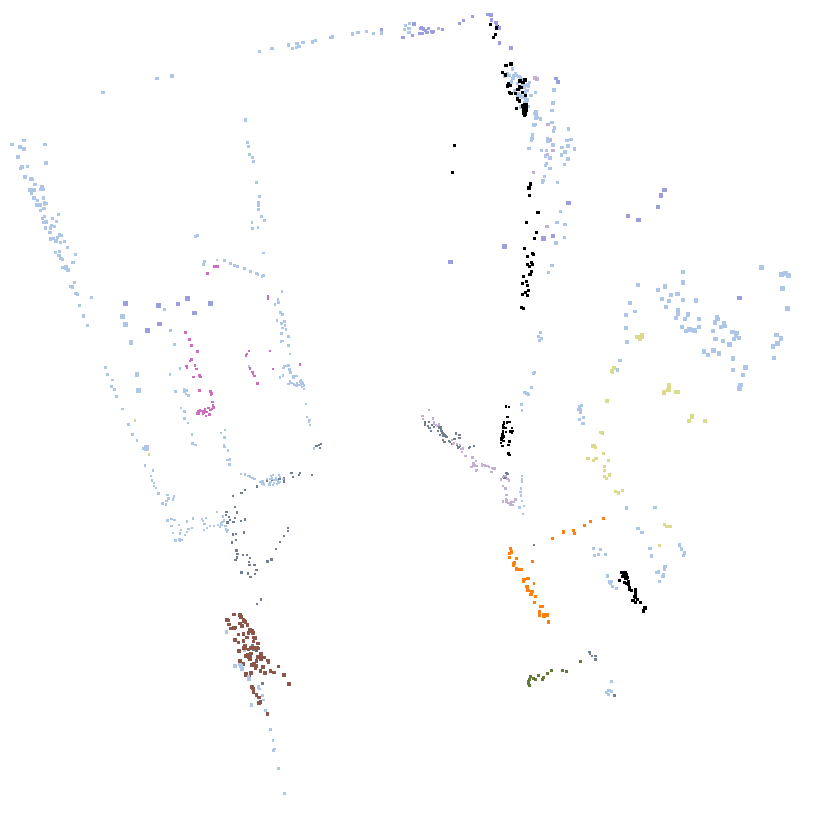
\includegraphics[width=\textwidth]{ply_log-model_1bG-gsbb_3B1-bs25-lr1-ds_30-xyz_midnorm_block-color_1norm-nxnynz-12800-mat_1083/17DRP5sb8fy_1_2_a946/err00.png}
	\caption{err}
\end{subfigure}
	\caption{17DRP5sb8fy\_1\_2\_a946}
\end{figure}

\begin{figure}[H]
	\centering
	\begin{subfigure}[h]{0.5\textwidth}
	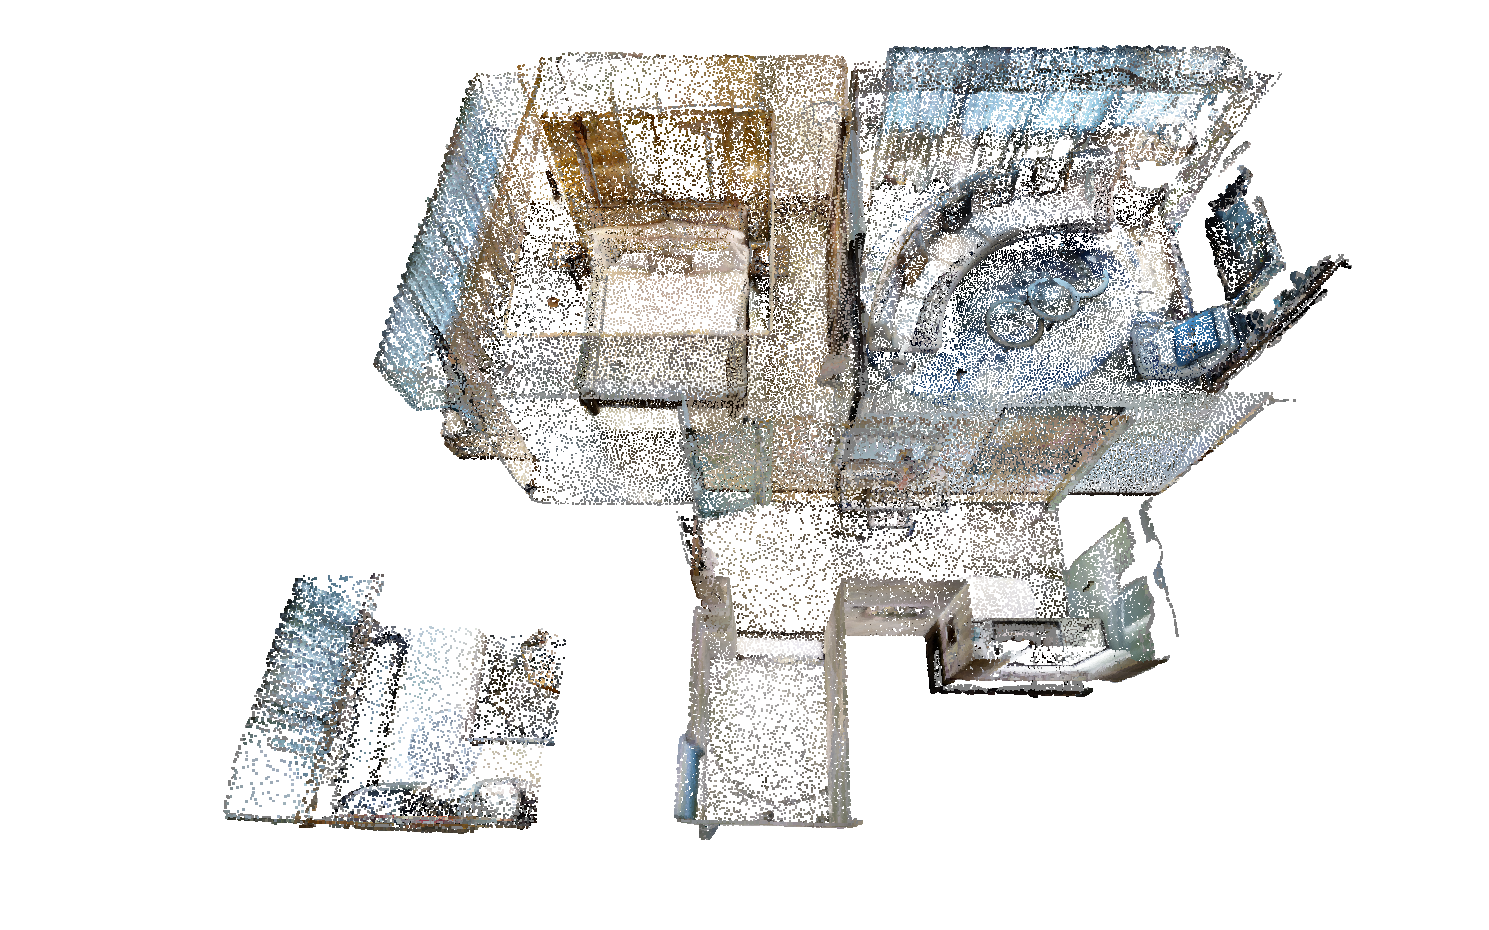
\includegraphics[width=\textwidth]{ply_log-model_1bG-gsbb_3B1-bs25-lr1-ds_30-xyz_midnorm_block-color_1norm-nxnynz-12800-mat_1083/17DRP5sb8fy_0_25_a946/raw00.png}
	\caption{colorized point cloud}
	\end{subfigure}
	\begin{subfigure}[h]{0.49\textwidth}
	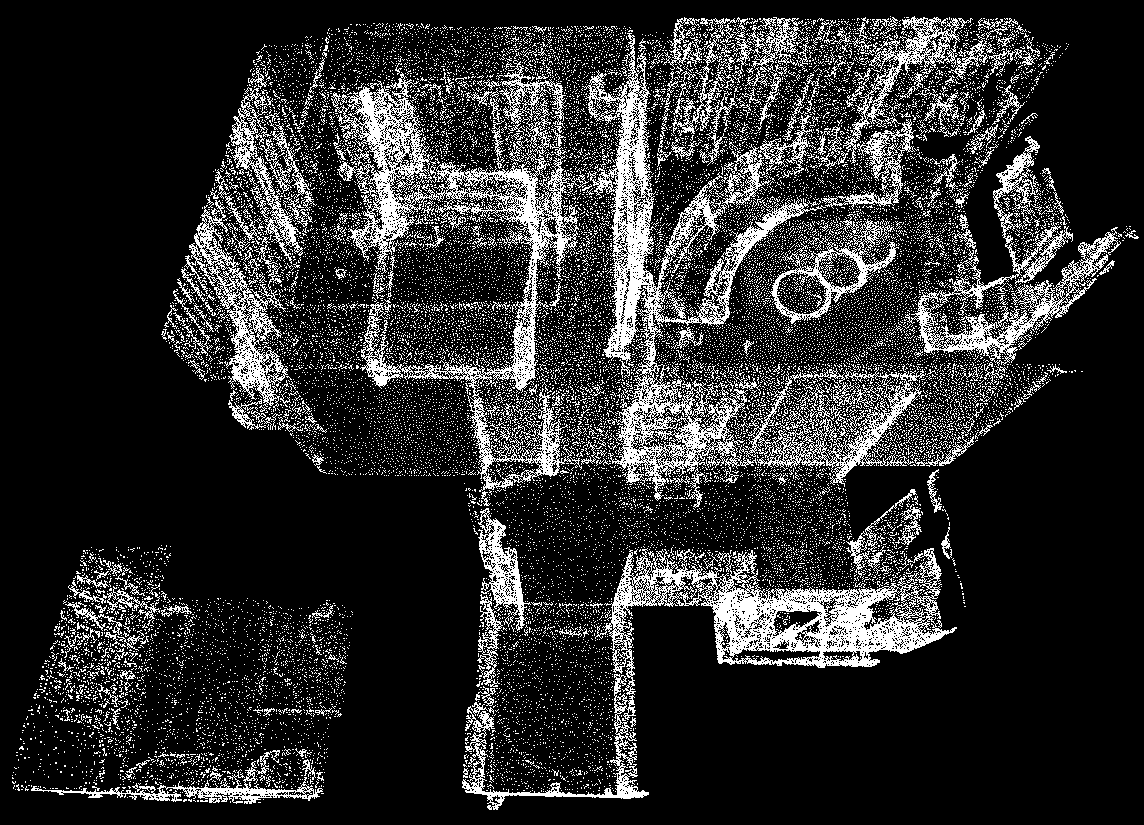
\includegraphics[width=\textwidth]{ply_log-model_1bG-gsbb_3B1-bs25-lr1-ds_30-xyz_midnorm_block-color_1norm-nxnynz-12800-mat_1083/17DRP5sb8fy_0_25_a946/xyz00.png}
	\caption{raw point cloud}
	\end{subfigure}
	\begin{subfigure}[h]{0.5\textwidth}
		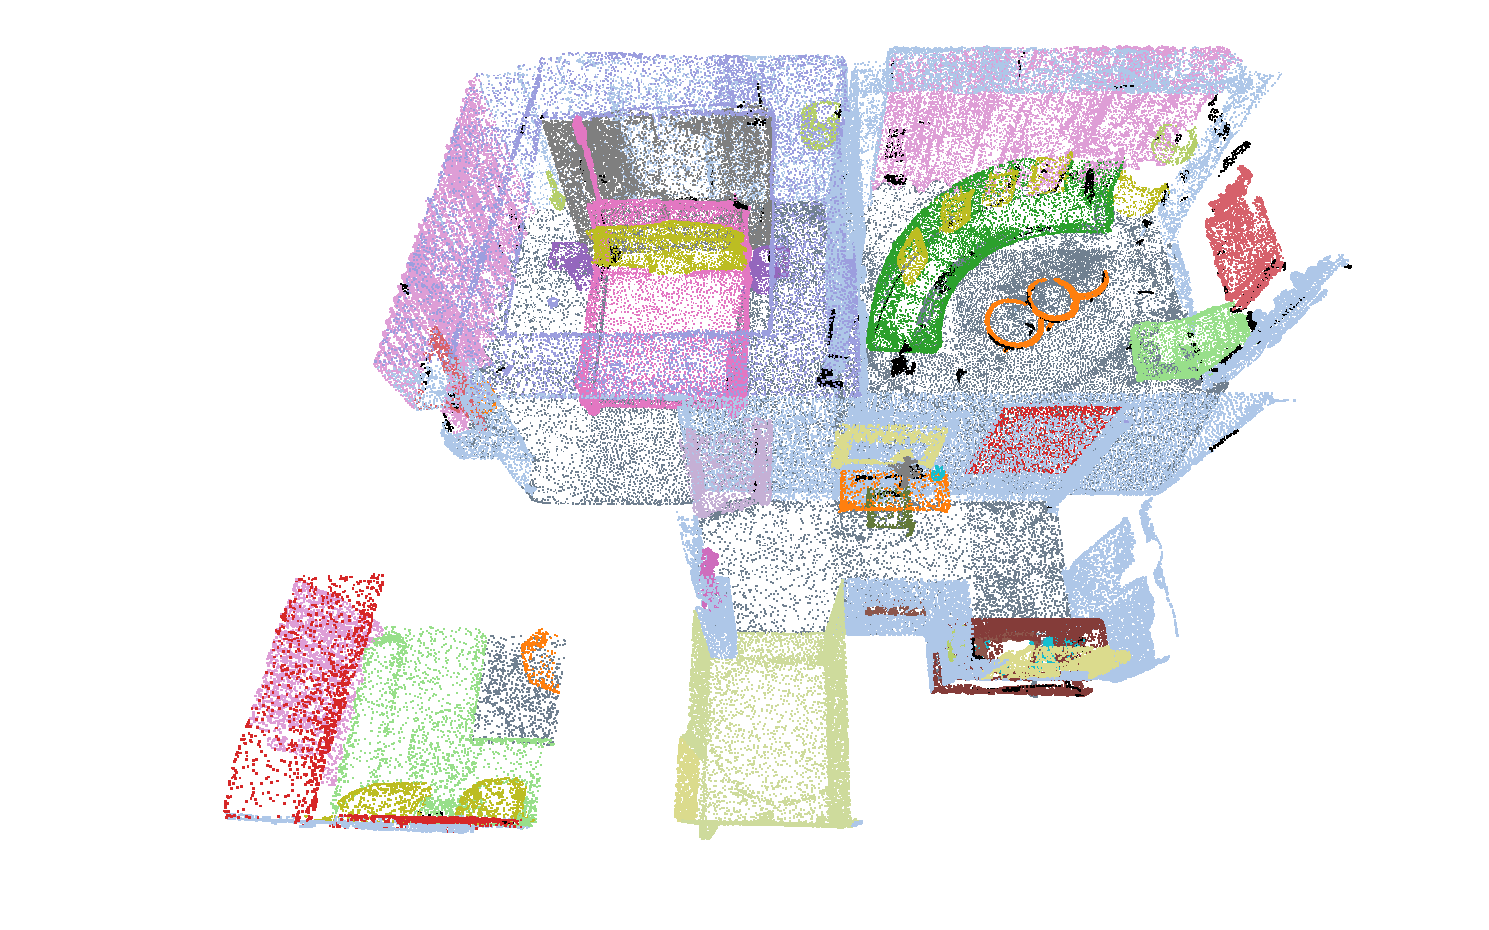
\includegraphics[width=\textwidth]{ply_log-model_1bG-gsbb_3B1-bs25-lr1-ds_30-xyz_midnorm_block-color_1norm-nxnynz-12800-mat_1083/17DRP5sb8fy_0_25_a946/gt00.png}
		\caption{gt}
	\end{subfigure}
	\begin{subfigure}[h]{0.49\textwidth}
		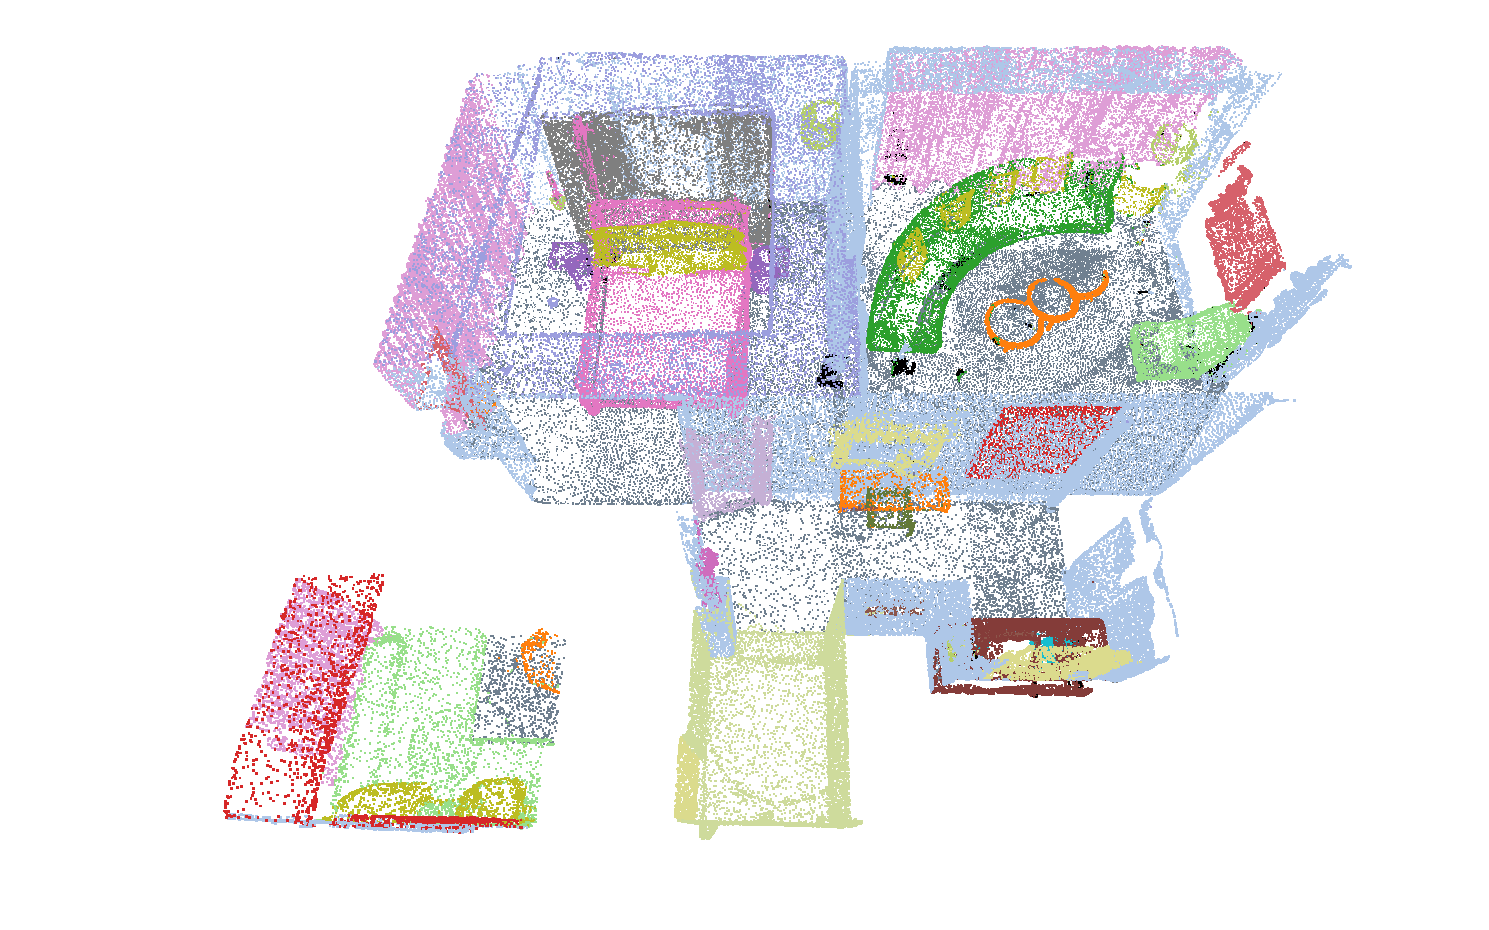
\includegraphics[width=\textwidth]{ply_log-model_1bG-gsbb_3B1-bs25-lr1-ds_30-xyz_midnorm_block-color_1norm-nxnynz-12800-mat_1083/17DRP5sb8fy_0_25_a946/pred00.png}	
		\caption{pred}
	\end{subfigure}
	\begin{subfigure}[h]{0.5\textwidth}
		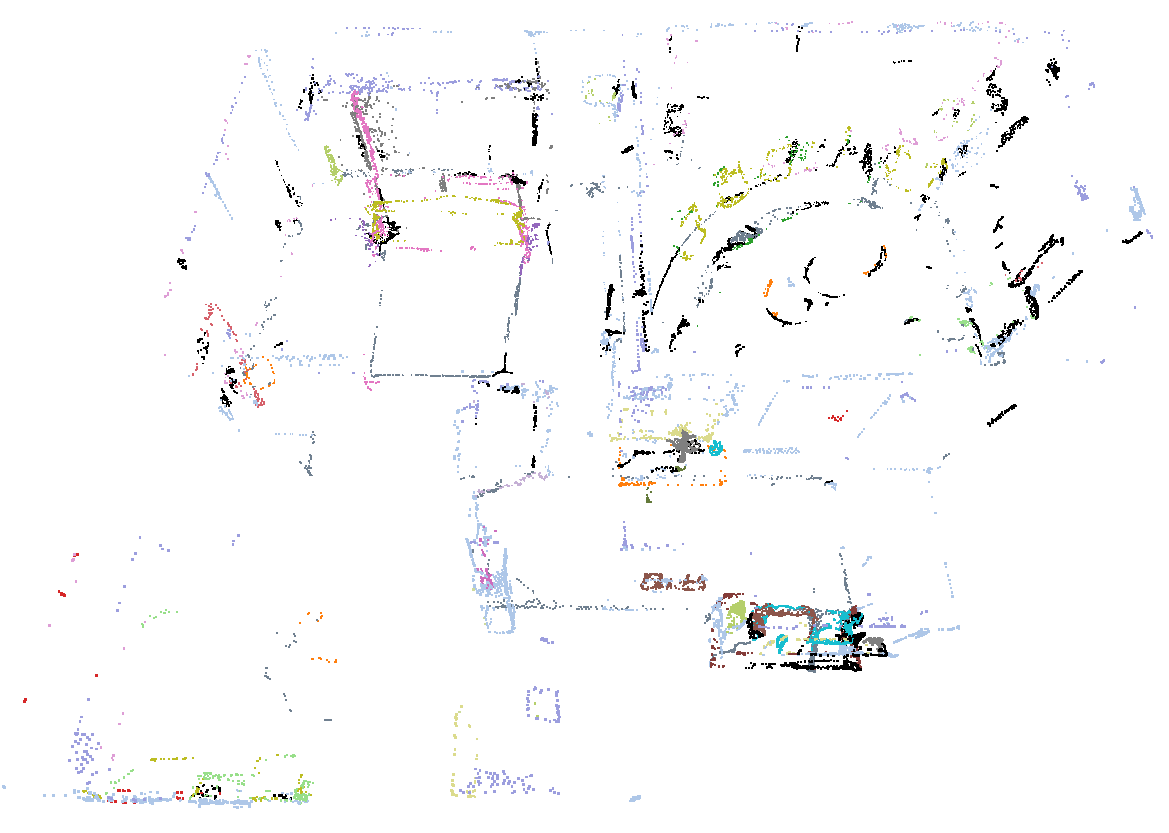
\includegraphics[width=\textwidth]{ply_log-model_1bG-gsbb_3B1-bs25-lr1-ds_30-xyz_midnorm_block-color_1norm-nxnynz-12800-mat_1083/17DRP5sb8fy_0_25_a946/err00.png}
		\caption{err}
	\end{subfigure}
	\caption{17DRP5sb8fy\_0\_25\_a946}
\end{figure}

\subsubsection{bad: 18737,eval 0.071}
model: 1bG \par
sampling \& grouping: stride\_0d1\_step\_0d1\_bmap\_nh5\_12800\_1d6\_2\_fmn3-512\_64\_24-48\_16\_12-0d2\_0d6\_1d2-0d2\_0d6\_1d2 \par
batch size: 25 \par
learning rate: 0.001000 \par
decay\_epoch\_step: 50 \par
epoch 0 train IsShuffleIdx: True  \par
epoch 0 train IsShuffleIdx: True  \par
matterport3d  \par
feed\_data\_elements:['xyz\_midnorm\_block', 'color\_1norm', 'nxnynz'] \par 
feed\_label\_elements:['label\_category', 'label\_instance']  \par
train data shape: [18737 12800     9]    \par
test data shape: [ 4172 12800     9] \par

\begin{figure}[H]
	\centering
	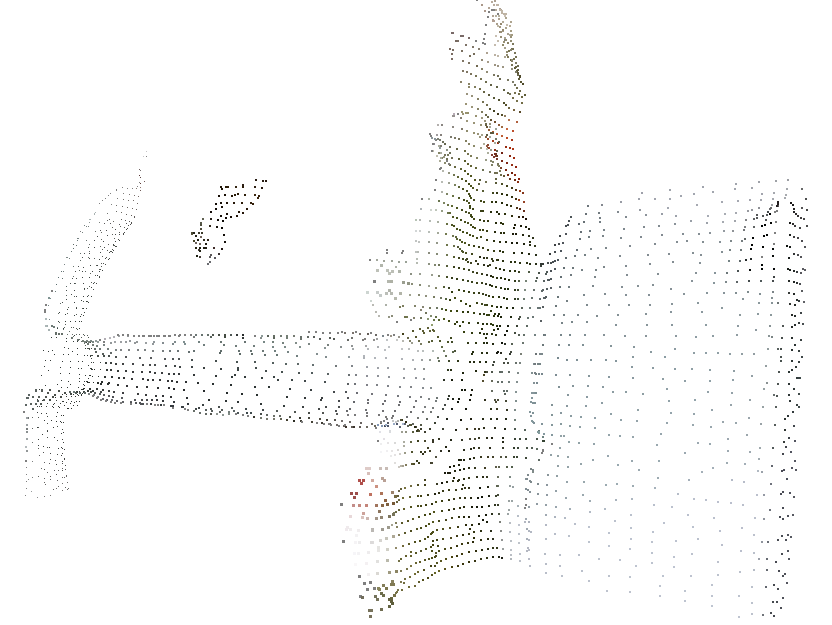
\includegraphics[width=0.49\textwidth]{ply_log-model_1bG-gsbb_3B1-bs25-lr1-ds_50-Sf_Y-xyz_midnorm_block-color_1norm-nxnynz-12800-mat_18737/qoi_r1Q_r47_rPc_rqf_2_3_raw00.png}
	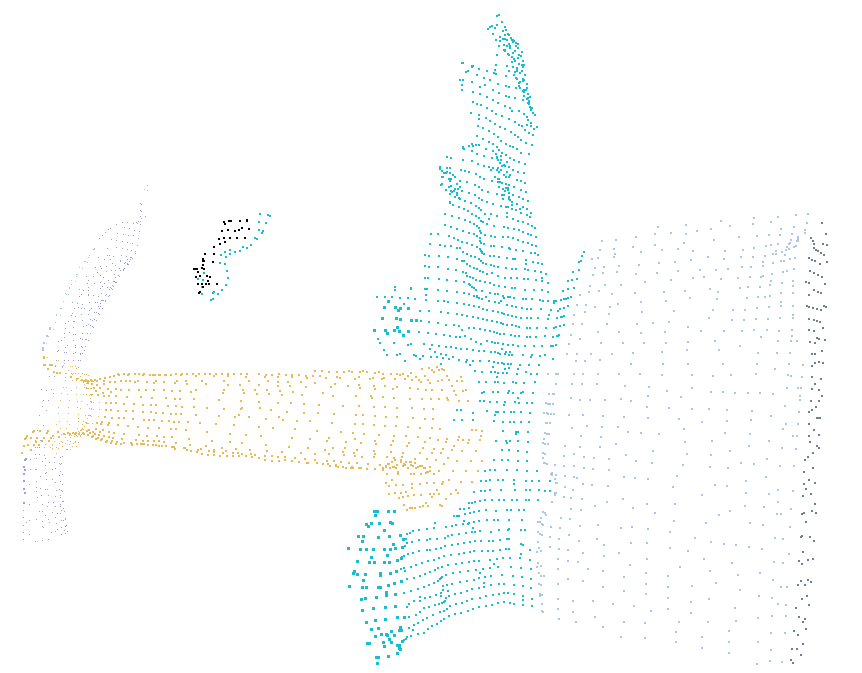
\includegraphics[width=0.49\textwidth]{ply_log-model_1bG-gsbb_3B1-bs25-lr1-ds_50-Sf_Y-xyz_midnorm_block-color_1norm-nxnynz-12800-mat_18737/qoi_r1Q_r47_rPc_rqf_2_3_gt00.png}
	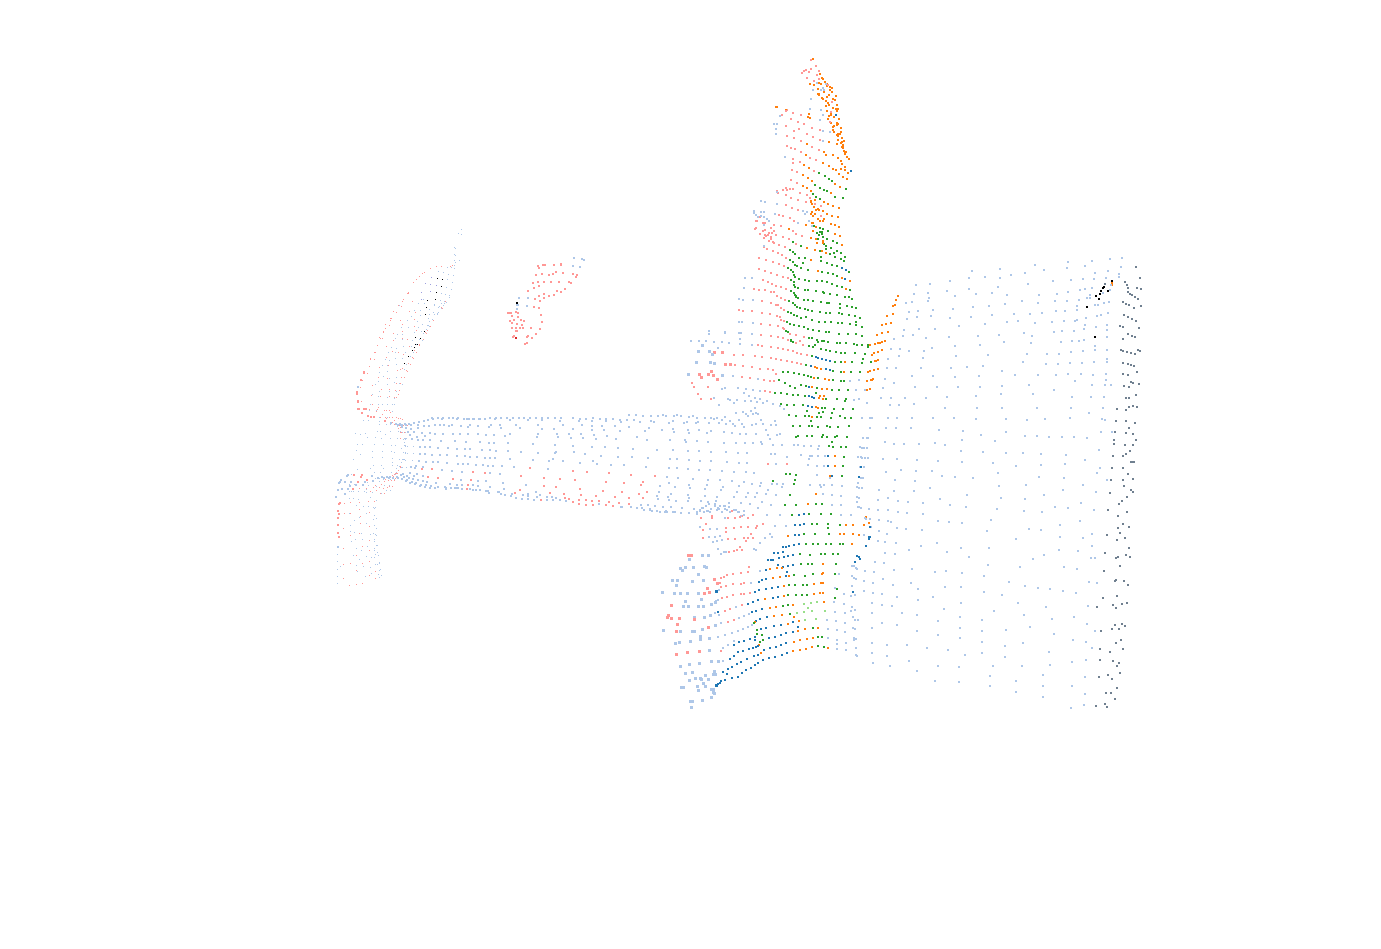
\includegraphics[width=0.49\textwidth]{ply_log-model_1bG-gsbb_3B1-bs25-lr1-ds_50-Sf_Y-xyz_midnorm_block-color_1norm-nxnynz-12800-mat_18737/qoi_r1Q_r47_rPc_rqf_2_3_pred00.png}
	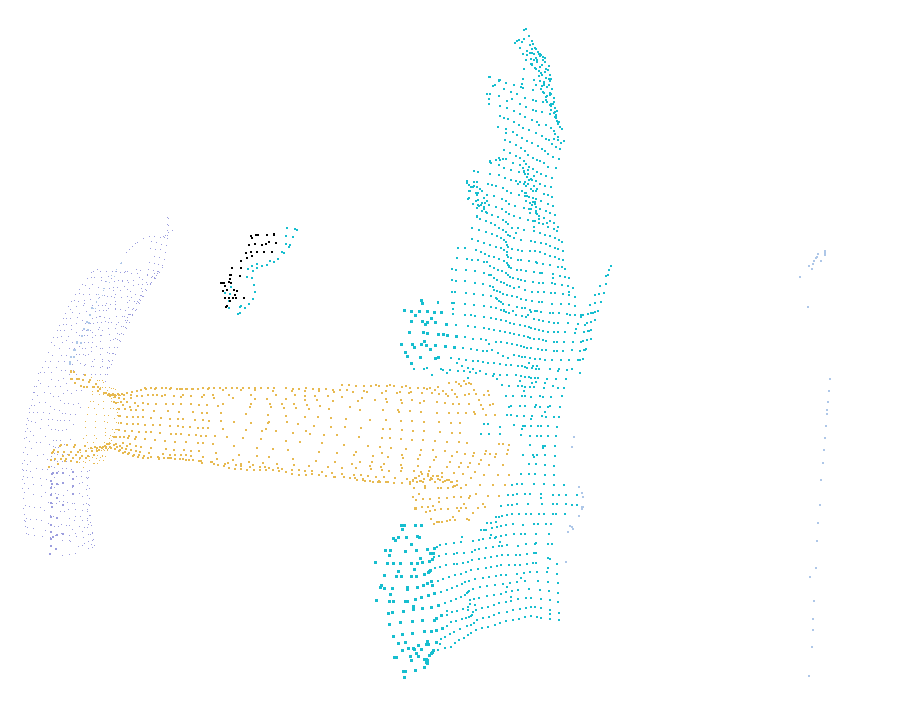
\includegraphics[width=0.49\textwidth]{ply_log-model_1bG-gsbb_3B1-bs25-lr1-ds_50-Sf_Y-xyz_midnorm_block-color_1norm-nxnynz-12800-mat_18737/qoi_r1Q_r47_rPc_rqf_2_3_a0d071_err00.png}
	
\includegraphics[width=0.49\textwidth]{ply_log-model_1bG-gsbb_3B1-bs25-lr1-ds_50-Sf_Y-xyz_midnorm_block-color_1norm-nxnynz-12800-mat_18737/qoi_r1Q_r47_rPc_rqf_2_3_a0d071_crt00.png}
	\caption{qoi\_r1Q\_r47\_rPc\_rqf\_2\_3\_a0d071 (raw,gt,pred,err,crt)}
\end{figure}


\subsection{point++}
\subsubsection{scannet seg}

\begin{center}
	\centering \def\arraystretch{1.5} \small
	\begin{tabular}{|p{1.5cm} | p{2cm} | p{3.5cm} || p{5cm}|} 
		\hline
		\multicolumn{4}{|c|}{each room as a block, total 40 block}\\
		\hline
		batch size\par batch num & lr\par ds & data elements & epoch-point ac-class ac \par train/eval/eval whole scene \\
		\hline
		30/40 & 0.001 & xyzmid & 200-0.675/0.757-0.54/0.799-0.52\\
		\hline
		25 & 0.001 & xyzmid & 200-0.689/0.787-0.556/0.815-0.517i\\
		\hline
	\end{tabular}
\end{center}


\subsection{whole room global block \& multi scales \& scan 305}
\begin{tabular}{|p{1.5cm}|p{1.5cm}|p{1cm}|p{2cm}|p{1.5cm}|p{6cm}| }
	\hline
	\multicolumn{6}{|p{12cm}|}{nh5: stride\_0d1\_step\_0d1\_pl\_nh5-1d6\_2/ \par bxmh5:  stride\_0d1\_step\_0d1\_bxmh5-12800\_1d6\_2\_fmn4-480\_80\_24-80\_20\_10-0d2\_0d6\_1d2-0d2\_0d6\_1d2-3A1 \par eval: 17D\_1LX\_1pX\_29h\_2az } \\
	\hline
	model & bs/bn& lr-decay & elements & loss weight\par in drop & epoch-pacc-cacc train/eval \\
	\hline
	5bG\_114 & 6/40 &2-30 & xyz midnorm\par color& E\par N &100-0.805-0.645\par 200-0.865-0.708 \par 300-0.880-0.773  \\
	\hline
	5aG\_114 & 2/140 &2-30 & xyz midnorm\par color& E\par N &100-0.802-0.619\par 200-0.873-0.694 \par 300-0.895-0.784  \\
	\hline
	5aG\_114 & 2/140 &2-30 & xyz midnorm\par color& E\par idp5 &100-0.807-0.687\par 200-0.877-0.729 \par 300-0.895-0.778  \\
	\hline
	
	\multicolumn{6}{|p{12cm}|}{ Conclusion:\par	(1) Nein 114 is better than 111  } \\
	\hline
\end{tabular}	


\subsection{Sparse voxel net}
\subsubsection{90000}
\begin{tabular}{|p{1.5cm}|p{1.5cm}|p{1cm}|p{1.5cm}|p{1.5cm}|p{1.5cm}|p{5cm}| }
	\hline
	\multicolumn{7}{|p{14cm}|}{nh5: 90000\_gs-3d6\_-6d3/ \par bxmh5:  90000\_gs-3d6\_-6d3\_fmn1444-6400\_2400\_320\_32-32\_16\_32\_48-0d1\_0d3\_0d9\_2d7-0d1\_0d2\_0d6\_1d8-pd3-mbf-4A1 \par eval: test } \\
	\hline
	model & bs/bn& lr-decay & elements & norm innet\par aug & loss weight\par in drop & epoch-pacc-cacc train/eval \\
	\hline
		
	5VaG\_114 & 16/113 &1-50 & xyz mid & No & Num lw\par dp:3N5\par N shuffle &20-0.764-0.556/0.645-0.362\par 40-0.864-0.695/0.675-0.351\par 100-0.935-0.842/0.682-0.380\par 200-0.961-0.897/0.671-0.374\par 300-0.969-0.920/0.676-0.360  \\
	\hline
	5VaG\_114 & 30/40 &2-40 & xyz mid\par color & No  & Num lw\par dp:466\par Y shuffle &20-0.605-0.443/0.577-0.381\par 40-0.668-0.490/0.544-0.372 \par 100-0.795-0.581/0.653-0.384\par 120-0.805-0.594/0.676-0.377  \\
	\hline
	5VaG\_114 & 30/40 &2-40 & xyz mid\par color & No  & Num lw\par dp:4N6\par Y shuffle &20-0.677-0.520/0.607-0.373\par 40-0.801-0.624/0.659-0.373 \par 100-0.906-0.754/0.687-0.368\par 120-0.911-0.776/0.692-0.421  \\
	\hline
	5VaG\_114 & 30/40 &2-40 & xyz mid\par color & No  & Num lw\par dp:N66\par Y shuffle &20-0.614-0.457/0.566-0.344\par 40-0.685-0.500/0.552-0.356 \par 60-0.741-0.552/0.650-0.357\par 80-0.770-0.564/0.649-0.392\par 98-0.797-/0.675  \\
	\hline
	
	5VaG\_114 & 30/40 &2-40 & xyz mid\par color & Mid & Num lw\par dp:555\par Y shuffle &100-0.746/0.649\par 300-0.823-0.608/0.682-0.377\\
	\hline
	5VaG\_114 & 39/40 &2-40 & xyz mid\par color & Mid & Num lw\par dp:5N5\par Y shuffle &40-0.839-0.649/0.656-0.353\par 100-0.918-0.771/0.681-0.381\par\\
	\hline
	5VaG\_114 & 36/40 &1-40 & xyz mid\par color & Mid & Num lw\par dp:NN5\par Y shuffle &40-0.833-0.655/0.628-0.329\par 100-0.916-0.772/0.682-0.339\par 178-0.941/0.686\\
	\hline
	5VaG\_114 & 7/240 &2-40 & xyz mid\par color & Mid \par Group Norm& Num lw\par dp:NN5\par Y shuffle &40-0.664/0.577\par 100-0.816-0.586\par 150-0.869-0.592\\
	\hline\hline
	5VaG\_114 & 9 &2-40 & xyz mid\par color & Rotate Ref & Num lw\par dp:NN5\par Y shuffle &40-0.787-0.620/0.662-0.401\par 100-0.907-0.755/0.699-0.410\par 200-0.939-0.816/0.6990.430\par 300-0.950-0.845/0.691-0.430\\
	\hline
	
	\multicolumn{7}{|p{14cm}|}{ Conclusion:\par	
		Mid norm in sub block seems worse than no. \par 
		The infuence of input drop seems not obvious. \par 
		Dropout of cnn (0.5) makes the net really hard to train. Seems no good for overfitting.\par 
		Group norm is poor.   } \\
	\hline
\end{tabular}	

\subsubsection{30000}
\begin{tabular}{|p{1.5cm}|p{1.5cm}|p{1cm}|p{1.5cm}|p{1.5cm}|p{1.5cm}|p{5cm}| }
	\hline
	\multicolumn{7}{|p{14cm}|}{bxmh5: 30000\_gs-2d4\_-3d4\_fmn1444-2048\_1024\_128\_24-48\_32\_48\_27-0d1\_0d4\_1\_2d2-0d1\_0d2\_0d6\_1d2-pd3-mbf-4B1  \par eval: test \par Void point id deleted} \\
	\hline
	model & bs& lr-decay & elements & norm innet\par aug & loss weight\par in drop & epoch-pacc-cacc train/eval \\
	\hline
	
	5VaG\_114 & 9 &2-40 & xyz mid\par color & Rotate Ref & Num lw\par dp:5N5\par Y shuffle & 20-0.749/0.645\par 30-0.810/0.705\par 40-0.870/0.744\par 80-0.917-0.737/0.7540.422\par 120-0.929-0.765\par 200-0.953-0.774\par 300-0.962/0.774\\
	\hline
	\multicolumn{7}{|p{14cm}|}{ 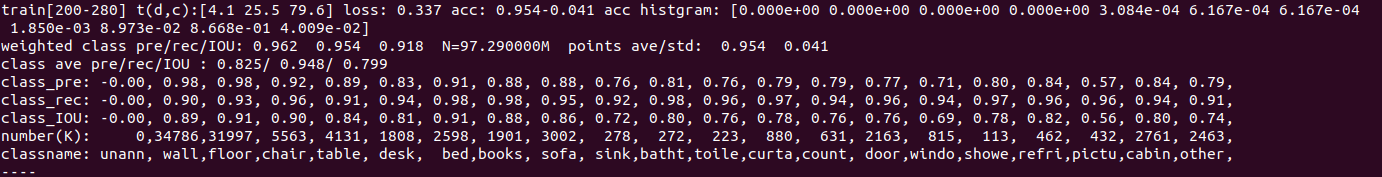
\includegraphics[width=\textheight]{images/svoxel/novoid/train} \par 
	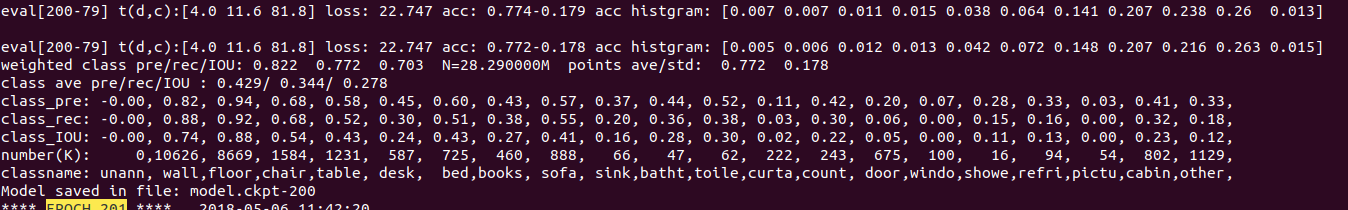
\includegraphics[width=\textheight]{images/svoxel/novoid/test}} \\
	\hline
	
	\multicolumn{7}{|p{14cm}|}{ Conclusion:\par	 } \\
	\hline
\end{tabular}


\subsection{My point++}	
\emph{After fix shuffle problem}
\subsubsection{MODELNET40}
\begin{tabular}{|p{1.5cm}|p{1.5cm}|p{1cm}|p{1.5cm}|p{1.5cm}|p{1.5cm}|p{5cm}| }
	\hline
	\multicolumn{7}{|p{14cm}|}{bxmh5:1024\_gs3\_3\_fmn1444-1024\_320-24\_32-0d2\_0d4-0d1\_0d2-pd3-2M1\par 
	No block merging. Replicate redundant. }\\
	\hline
	
	model & bs& lr\par bn decay & elements & norm innet\par aug & loss weight\par in drop & epoch-pacc-cacc train/eval \\
	\hline
	
	3m & 32\par 40 after epoch 100 & 1-30 \par 5-5 & xyz-mid & mid, Rotate Ref & E, NN5 &1-0.355/0.375\par 4-0.504/0.544\par 10-0.603/0.640\par 30-0.742/0.759\par 50-0.798/0.804\par 60-0.834/0.823 \par 80-0.869/0.844\par 100-0.893/0.847  \\
	\hline
	3m & 32 & 1-30 \par 7-7 & xyz-mid & mid, Rotate Ref & E, NN5 & 10-0.636/0.684\par 50-0.851/0.826  \\
	\hline
	3m & 32 & 1-30 \par 5-5 & xyz & mid, Rotate Ref & E, NN5 &1-0.589/0.629\par 2-0.648/0.680\par 4-0.713/0.714\par 10-0.807/0.761\par 30-0.942/0.795\par 60-0.982/0.804 \\
	\hline
	
	\multicolumn{7}{|p{14cm}|}{ Conclusion:\par	
	(1) Global mid normalized xyz input reduces the learning speed, but can reduce overfitting. Why this makes a significant difference, considering mid norm is applied to each scale. } \\
	\hline
\end{tabular}

	
\end{document}